\documentclass[12pt,letterpaper]{report}

\usepackage[margin=1in]{geometry}
\usepackage[T1]{fontenc}
\usepackage[utf8]{inputenc}
\usepackage{lmodern}
\usepackage{microtype}
\usepackage{setspace}
\usepackage{booktabs}
\usepackage{tabularx}
\usepackage{longtable}
\usepackage{array}
\usepackage{multirow}
\usepackage{amsmath,amssymb,mathtools}
\usepackage{enumitem}
\usepackage{xcolor}
\usepackage{hyperref}
\usepackage{xurl}
\usepackage[nameinlink,noabbrev]{cleveref}
\usepackage{tikz}
\usetikzlibrary{arrows.meta,positioning,shapes.geometric,fit,calc,backgrounds}
\usepackage{pgfplots}
\pgfplotsset{compat=1.18}
\usepackage{caption}
\usepackage{float}
\usepackage{fancyhdr}

\hypersetup{
  colorlinks=true,
  linkcolor=black,
  citecolor=black,
  urlcolor=blue,
  pdftitle={SkillLLM_v2: Provenance-Aware Skill Extraction and Contextual Career Intelligence},
  pdfauthor={Author name to be supplied for formal submission}
}
\setstretch{1.22}
\setlength{\parskip}{0.35em}
\setlength{\parindent}{1.5em}
\setlist[itemize]{leftmargin=2em,itemsep=0.18em,topsep=0.3em}
\setlist[enumerate]{leftmargin=2em,itemsep=0.18em,topsep=0.3em}
\captionsetup{font=small,labelfont=bf}
\pagestyle{fancy}
\fancyhf{}
\fancyhead[LE,RO]{\thepage}
\fancyhead[LO]{\nouppercase{\rightmark}}
\fancyhead[RE]{\nouppercase{\leftmark}}
\renewcommand{\headrulewidth}{0.3pt}
\setcounter{tocdepth}{2}
\setcounter{secnumdepth}{3}

\definecolor{implemented}{HTML}{DCEFE2}
\definecolor{experimental}{HTML}{FFF1C2}
\definecolor{future}{HTML}{E7E7E7}
\definecolor{anchor}{HTML}{DCE8F5}
\definecolor{ink}{HTML}{263238}
\tikzset{
  node/.style={draw=ink,rounded corners=2pt,align=center,font=\footnotesize,minimum height=7mm,inner sep=3.2pt},
  impl/.style={node,fill=implemented},
  exp/.style={node,fill=experimental},
  plan/.style={node,fill=future,dashed},
  anchorbox/.style={node,fill=anchor,very thick},
  data/.style={node,fill=white},
  flow/.style={-{Stealth[length=2.1mm]},thick,draw=ink},
  dashedflow/.style={-{Stealth[length=2.1mm]},thick,dashed,draw=ink}
}
\newcommand{\implementedlabel}{\textcolor{black}{\fcolorbox{ink}{implemented}{\strut implemented}}}
\newcommand{\experimentallabel}{\textcolor{black}{\fcolorbox{ink}{experimental}{\strut experimental}}}
\newcommand{\plannedlabel}{\textcolor{black}{\fcolorbox{ink}{future}{\strut planned / unevaluated}}}
\newcommand{\codepath}[1]{\nolinkurl{#1}}
\newcommand{\inlinecode}[1]{\texttt{\detokenize{#1}}}
\newcommand{\metric}[1]{\ensuremath{#1}}

\begin{document}
\pagenumbering{roman}
\begin{titlepage}
  \centering
  \vspace*{1.1in}
  {\Large\bfseries SkillLLM\_v2: Provenance-Aware Skill Extraction,\par}
  \vspace{0.12in}
  {\Large\bfseries Normalization, and Contextual Career Intelligence\par}
  \vspace{0.65in}
  {\large Technical Research Report\par}
  \vspace{0.24in}
  {\large Prepared for CSC 895 / CSC 898 and Professor Chen\par}
  \vfill
  {\large San Francisco State University\par}
  {\large Department of Computer Science\par}
  \vspace{0.35in}
  {\large September 2026\par}
  \vspace{0.35in}
  \begin{minipage}{0.84\textwidth}\small
  \textbf{Administrative note.} This research report is thesis-quality but is not a signed submission copy. The author name, final course designation, committee information, and approval-page format must be confirmed with the department before formal submission.
  \end{minipage}
\end{titlepage}

\chapter*{Abstract}
\addcontentsline{toc}{chapter}{Abstract}
Skill extraction is a prerequisite for systems that compare a person's evidence-backed capabilities with job requirements and learning opportunities. Yet a useful extraction system must do more than emit plausible labels: it must preserve the source span, distinguish hard and soft skills, remain robust when auxiliary components disagree, and expose enough provenance for later matching and recommendation. This report presents SkillLLM\_v2, a modular research system for span-level skill extraction, canonicalization, profile construction, graph-structured explanation, job matching, and course recommendation.

The central extraction component is a Mistral Small 3.1 24B Instruct model adapted with a low-rank adapter on the local SkillSpan export. The audited 80-epoch, two-GPU run obtains exact-span F1 of 0.670069, token F1 of 0.787886, hard-skill F1 of 0.726450, and soft-skill F1 of 0.604046 on its persisted full-test artifact. In the same evaluation record, the BERT and zero-shot GLiNER baselines achieve exact-span F1 of 0.059150 and 0.075833 respectively. These results make the adapted Mistral model the extraction anchor rather than evidence that adding more modules automatically improves performance.

SkillLLM\_v2 therefore uses provenance-aware, non-regressive composition. Candidate merging protects anchor spans, taxonomy linking is attach-only, and a gate selects wrapper predictions only when they stay within configured exact-span and soft-skill tolerances. The full wrapper is accepted as non-regressive and records exact-span F1 of 0.671102, but the difference is small and does not establish a general improvement claim. The implementation also constructs evidence-preserving profile summaries, deterministic cached context packets, and an in-memory skill graph. These downstream paths are implemented and smoke-tested; however, labelled job-ranking and course-ranking evaluations are unavailable, so no effectiveness claim is made for them.

The report contributes a detailed code-to-artifact audit, a transparent experimental account, reproducible system diagrams, and a research finding of practical importance: a modular career-intelligence pipeline should treat high-quality extraction as an invariant to protect, while using normalization, context, and graph components to enrich provenance and explanation rather than silently rewriting reliable spans.


\chapter*{Acknowledgements}
\addcontentsline{toc}{chapter}{Acknowledgements}
This report was prepared for the SkillLLM\_v2 research update. The author thanks Professor Chen for guidance on the scope of the culminating research deliverable and the contributors of the SkillSpan benchmark for making span-level hard- and soft-skill evaluation possible.

\tableofcontents
\listoffigures
\listoftables

\chapter*{Abbreviations}
\addcontentsline{toc}{chapter}{Abbreviations}
\begin{longtable}{p{0.18\textwidth}p{0.72\textwidth}}
\toprule
Term & Meaning \\
\midrule
\endhead
CAG & Cache-augmented context in the SkillLLM\_v2 implementation \\
DDP & Distributed data parallel training \\
F1 & Harmonic mean of precision and recall \\
GLiNER & Generalist model for open-label named-entity recognition \\
LoRA & Low-rank adaptation \\
NER & Named-entity recognition \\
PEFT & Parameter-efficient fine-tuning \\
RAG & Retrieval-augmented generation \\
SFT & Supervised fine-tuning \\
\bottomrule
\end{longtable}

\clearpage
\pagenumbering{arabic}
\chapter{Introduction}
\label{ch:introduction}

\section{Motivation}

Job advertisements, resumes, course descriptions, and career histories all describe capabilities in natural language. A person may write ``built data pipelines in Python and SQL,'' a vacancy may request ``cloud deployment and stakeholder communication,'' and a course description may state that it teaches distributed systems. A career-support system cannot reliably compare these texts by string overlap alone. The terms may be abbreviated, may refer to the same canonical capability through aliases, and may encode different evidence strengths. At the same time, a system that invents a capability, loses the text span that justified it, or modifies a correct prediction while attempting to normalize it creates an error that propagates to matching and recommendation.

Skill extraction is therefore a useful intermediate representation for computational labour-market analysis. SkillSpan formalizes the task as span-level identification of hard and soft skills in English job postings and supplies expert annotation guidelines rather than a fixed inventory-only label space~\cite{zhang2022skillspan}. Recent surveys position this task at the intersection of information extraction, taxonomy alignment, and labour-market analysis~\cite{senger2024survey}. The local SkillSpan export is particularly suitable for a research system because it retains tokens, two skill-related BIO tag sequences, document delimiters, and a source field. It permits a span-focused comparison in which surface form, boundaries, and label must all be handled explicitly.

Large language models make structured extraction attractive because one model can produce a variable number of typed spans in a JSON schema. However, a generative output is not automatically an auditable record. It can include paraphrases instead of substrings, fail to parse, produce ambiguous labels, or make a broadly reasonable but unsupported inference. Classical and neural sequence labellers have complementary properties: they are often tied to a fixed labelling interface and can be evaluated directly at token or span level, but they do not by themselves solve canonicalization, evidence preservation, or downstream context construction. The design challenge is thus not simply to add components around an LLM. It is to make every component safe with respect to the strongest available extraction evidence.

This report documents SkillLLM\_v2, a codebase that implements a Mistral LoRA extraction path, auxiliary GLiNER and dictionary candidates, provenance-aware merging, rule-based verification and calibration interfaces, attach-only taxonomy linking, structured profile compaction, in-memory graph construction, deterministic matching, course recommendation, and artifact gates. The report treats these as distinct claims. Some are evaluated with persisted full-test extraction metrics; some are exercised by unit tests and demo artifacts; and some remain future evaluation work. This separation matters in an advisor-facing report because a runnable architectural path is valuable, but it is not equivalent to a validated product outcome.

\begin{figure}[H]
\centering
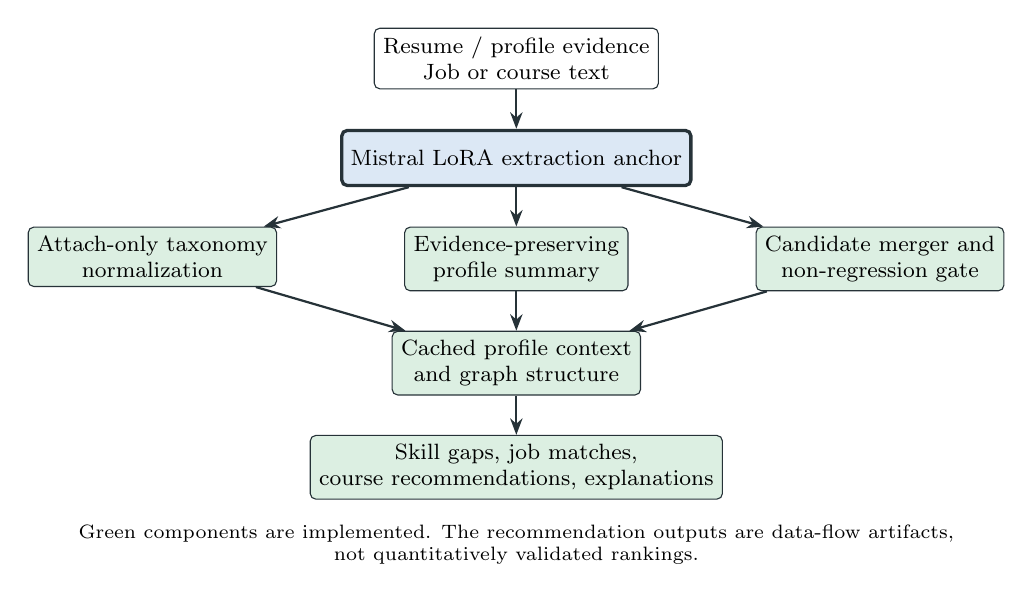
\begin{tikzpicture}[node distance=5mm and 8mm]
\node[data] (input) {Resume / profile evidence\\Job or course text};
\node[anchorbox,below=of input] (extract) {Mistral LoRA extraction anchor};
\node[impl,below left=of extract] (norm) {Attach-only taxonomy\\normalization};
\node[impl,below=of extract] (profile) {Evidence-preserving\\profile summary};
\node[impl,below right=of extract] (policy) {Candidate merger and\\non-regression gate};
\node[impl,below=of profile] (context) {Cached profile context\\and graph structure};
\node[impl,below=of context] (outputs) {Skill gaps, job matches,\\course recommendations, explanations};
\draw[flow] (input)--(extract);
\draw[flow] (extract)--(norm);
\draw[flow] (extract)--(profile);
\draw[flow] (extract)--(policy);
\draw[flow] (norm)--(context);
\draw[flow] (profile)--(context);
\draw[flow] (policy)--(context);
\draw[flow] (context)--(outputs);
\node[below=2mm of outputs,font=\scriptsize,align=center] {Green components are implemented. The recommendation outputs are data-flow artifacts,\\not quantitatively validated rankings.};
\end{tikzpicture}

\caption{Overall SkillLLM\_v2 structure. The architecture distinguishes implemented local modules from unevaluated claims about recommendation effectiveness.}
\label{fig:overall}
\end{figure}

\section{Research problem}

The main problem addressed in this work is: \emph{How can a domain-adapted language model be combined with provenance-aware normalization and contextual structure without allowing downstream processing to silently degrade reliable span extraction?} This formulation intentionally places reliability before architectural breadth. It does not assume that a graph, retriever, verifier, or taxonomy linker improves F1 merely because it is present. Instead, it asks whether a high-quality anchor can remain the source of truth for extraction while other modules add canonical identifiers, evidence-bearing user memory, gap explanations, and bounded decision support.

The code and artifacts give a concrete reason for this framing. The persisted full-test Mistral LoRA artifact has exact-span F1 of 0.670069 and token F1 of 0.787886. The corresponding BERT and GLiNER artifacts score 0.059150 and 0.075833 exact-span F1. The full CAG/graph wrapper records 0.671102 exact-span F1, a difference of 0.001033 over the anchor. That small difference is inside the configured gate tolerance and is sufficient to support a non-regression decision in this snapshot; it is not sufficient evidence for a general claim that a complex wrapper improves extraction. A separate historical error-analysis report records substantial destructive boundary edits in an earlier path. The system design responds to that observation by preserving anchor candidates and by making fallback explicit.

\section{Research questions}

The report answers the following questions to the extent supported by local evidence.

\begin{enumerate}
  \item \textbf{RQ1:} How effectively does the persisted Mistral LoRA extraction path identify hard and soft skill spans in the local SkillSpan evaluation path?
  \item \textbf{RQ2:} How do the BERT baseline, zero-shot GLiNER baseline, and wrapper variants compare with the Mistral anchor under the stored metrics?
  \item \textbf{RQ3:} What implementation rules make auxiliary candidate generation, boundary refinement, verification, and normalization non-destructive with respect to anchor extraction?
  \item \textbf{RQ4:} What evidence-preserving representation can transform extracted skills into a compact profile and contextual packet suitable for later retrieval and explanation?
  \item \textbf{RQ5:} Which downstream graph, matching, and recommendation capabilities are implemented, and which still lack labelled outcome evaluation?
\end{enumerate}

These questions deliberately do not ask whether the system achieves better job matching or recommendation quality. The repository contains no relevance labels for such a claim: job nDCG@10 and course precision@5 are both recorded as unavailable. The design and implementation can be assessed now; ranking effectiveness must be assessed later with a labelled protocol.

\section{Contributions}

The first contribution is an evidence-led account of a two-GPU 80-epoch Mistral LoRA run over the local SkillSpan export. Its configuration, checkpoints, training summary, generated predictions, and metrics are persisted. The second is a provenance-aware candidate policy. Each valid skill record carries a surface form, label, offsets, source, confidence, evidence, canonical fields, and metadata. Mistral-originated candidates are protected; unanchored additions must clear configured confidence and alias-evidence conditions; and the wrapper gate compares candidate metrics with the anchor before choosing output predictions.

The third contribution is an implementation-level design for enriching extraction without conflating enrichment with accuracy. Taxonomy linking attaches information instead of rewriting offsets or labels. Profile summarization aggregates supplied extraction evidence rather than inferring hidden skills. Context compaction distinguishes stable cached information from dynamic job text and graph paths. The graph, matcher, gap detector, and recommender produce inspectable, deterministic records. Finally, the report contributes the audit in \codepath{docs/thesis/codebase\_audit.md}, system figures, a result table backed by JSON artifacts, and explicit limitations that prevent the thesis from overstating the current system.

\section{Thesis organization}

\Cref{ch:related-work} situates the project in skill extraction, span modelling, parameter-efficient adaptation, normalization, retrieval, and graph-based career systems. \Cref{ch:problem} defines the representations and metrics. \Cref{ch:architecture} maps the actual source tree to the system architecture. \Cref{ch:methodology} and \Cref{ch:experiments} describe data preparation, training, evaluation, and artifact handling. \Cref{ch:results} reports the verified metrics. \Cref{ch:error-analysis} discusses wrapper regression and the non-regression response. \Cref{ch:context} documents the profile, context, graph, and matching layers. The final chapters state limitations, future work, and conclusions.

\chapter{Background and Related Work}
\label{ch:related-work}

\section{Skill extraction and skill inventories}

Skill extraction identifies capability mentions in unstructured text. It is related to named-entity recognition, but the boundary of a skill can be long, compositional, and context dependent. A phrase such as ``experience with scalable distributed systems'' may include a tool, a concept, an experience qualifier, or several nested skills depending on the annotation rules. SkillSpan addresses this problem by annotating hard and soft skills at span level across 14.5K English job-posting sentences with more than 12.5K annotated spans~\cite{zhang2022skillspan}. It is particularly relevant here because the local export maintains the hard/soft distinction rather than collapsing all skills into one universal class.

Earlier systems connected extraction with normalization. The SKILL system treated identification and normalization as a linked problem at scale~\cite{zhao2015skill}; later work considers large-scale occupational normalization and extreme multi-label retrieval from job descriptions~\cite{hoang2018largescale,bhola2020retrieving}. This distinction is still important. Extraction answers whether a source says ``AWS,'' whereas normalization decides whether a surface form maps to a canonical concept such as Amazon Web Services. Conflating the two can hide an extraction error behind a plausible identifier. SkillLLM\_v2 adopts an explicit separation: its linker is attach-only, so canonicalization should not affect span-level extraction F1.

The Skill-LLM lineage demonstrates that general-purpose LLMs can be adapted for skill extraction~\cite{herandi2024skillllm}. Related job-market research explores LLM extraction, synthetic job-posting generation, and nearest-neighbour occupational skill extraction~\cite{nguyen2024rethinking,magron2024jobskape,zhang2024nnose}. These efforts motivate a generative JSON interface but do not remove the need for controlled local evaluation. In this report, the substantive model claim is limited to the stored Stage-2 Mistral results on the local data path, not a direct benchmark claim against papers using different pre-processing, model versions, or splits.

\section{Named-entity recognition and span modelling}

Sequence tagging is a useful baseline for extraction. BiLSTM-CRF and character-aware variants established effective NER architectures before transformer encoders~\cite{huang2015bilstmcrf,lample2016ner,ma2016bilstmcnncrf}. BERT made contextual token representations broadly available for downstream classification and sequence labelling~\cite{devlin2019bert}; RoBERTa and XLM-R extended the pre-training design space~\cite{liu2019roberta,conneau2020xlmr}. A BERT baseline is consequently an important control in this project, even though its local artifact is explicitly a CPU-fast baseline and does not match the Mistral result.

Span-specific methods emphasise that boundaries, not only token labels, determine correctness. SpanBERT pre-trains representations that focus on contiguous spans~\cite{joshi2020spanbert}, and SpanNER formulates recognition through span prediction~\cite{fu2021spanner}. DyGIE++ extends contextual span representations to entities, relations, and events~\cite{wadden2019dygiepp}. Such work is conceptually aligned with SkillSpan evaluation: a semantically reasonable phrase is still incorrect under exact matching when either boundary or label differs. SkillLLM\_v2 therefore reports exact, partial, token, hard-skill, and soft-skill metrics rather than relying on a single aggregate alone.

GLiNER is especially relevant as an auxiliary source because it supports generalist, open-label entity recognition with a bidirectional transformer~\cite{zaratiana2023gliner}. In the audited repository, however, the standalone GLiNER result is zero-shot/few-shot; fine-tuning was skipped. The thesis treats it as a recall-oriented candidate source and an honest baseline, not as evidence of a trained competitor. Generative approaches such as GPT-NER show that LLMs can produce entity structures directly~\cite{wang2023gptner}. Their principal risk in an extraction pipeline is not merely an invalid JSON string; it is a fluent string that fails to align to the input or rewrites a source span. The alignment and validation code in SkillLLM\_v2 address this operational issue.

\section{Domain adaptation and parameter-efficient fine-tuning}

Domain-adaptive pre-training and fine-tuning are common ways to transfer general language representations to specialised text~\cite{gururangan2020dontstop,howard2018ulmfit}. Full model adaptation is expensive for a large causal model, motivating parameter-efficient methods. LoRA freezes the base weights and introduces trainable low-rank update matrices~\cite{hu2022lora}. QLoRA combines adapter learning with quantized base-model loading and provides the NF4 and memory-management techniques that make 4-bit adaptation practical~\cite{dettmers2023qlora}. These papers motivate the compute-conscious method; they do not supply performance evidence for this particular model or corpus.

SkillLLM\_v2 uses a Mistral Small 3.1 24B Instruct path, a 4-bit configuration, and LoRA settings stored in YAML. The Mistral model family established a widely used open-weight architecture line~\cite{jiang2023mistral}, while the project-specific training summary supplies the more important claim here: a recorded 80-epoch, two-process run with persisted adapter and evaluation artifacts. The thesis differentiates this implemented training path from the broad PEFT literature. It does not assert that all hardware settings or all configurations from the cited work were reproduced.

\section{Taxonomy linking and retrieval}

Taxonomies make a skill representation more useful for aggregation, reporting, and matching. ESCO provides a semantic-interoperability framing for job matching~\cite{levrang2014esco}; ESCOXLM-R and entity-linking work show how job-market language can be related to structured inventories~\cite{zhang2023escoxlmr,zhang2024entitylinking}. Large language models have also been investigated as zero-shot ESCO skill matchers~\cite{clavie2023batteries}. A local implementation cannot be assumed to inherit the coverage or accuracy of those published systems. The audited Stage-2 code provides loaders and aliases for multiple sources, but its reported path is a custom alias-backed linker. Its 0.890 values are linked-candidate coverage, while a supervised canonical-link test set is absent.

Retrieval is relevant at two scopes. Dense passage retrieval~\cite{karpukhin2020dpr}, Sentence-BERT~\cite{reimers2019sentencebert}, SimCSE~\cite{gao2021simcse}, and ColBERT~\cite{khattab2020colbert} represent well-established semantic or late-interaction approaches. Retrieval-augmented generation combines retrieved evidence with a generator in knowledge-intensive tasks~\cite{lewis2020rag}. The project's `ContextualRetriever` is deliberately much smaller: it scores lexical term overlap over contextualised records. It serves a deterministic smoke/demo path and an interface boundary for future dense retrieval. This distinction prevents the report from labelling a lexical overlap class as a complete RAG evaluation.

\section{Graphs, matching, and contextual career intelligence}

Career systems need relationships that simple extraction does not express: a user has a skill; a job requires it; a course teaches it; a missing skill explains a weak match. Skills2Job demonstrates graph-oriented job recommendation~\cite{giabelli2021skills2job}. Person--job fit has also been studied through domain-adapted deep networks and context-aware transformer matching~\cite{bian2019domain,li2020competence}. These studies motivate the graph and matching interfaces in SkillLLM\_v2, but no paper can validate the repository's deterministic weights. The graph in this codebase is an in-memory NetworkX multigraph, and the matching result is an interpretable weighted formula.

Context management raises a different problem: sending an entire profile history with every query increases cost and can obscure fresh evidence. A compact, structured profile can cache stable, attributable facts while a retriever supplies dynamic job text. SkillLLM\_v2 labels this separation CAG/RAG/graph policy: stable profile summary, aliases, and course summaries are cached; job postings and scraped descriptions remain retrieval targets; relational explanations remain in the graph. This is a concrete design and smoke-tested implementation, not an empirical comparison of cache-augmented generation, RAG, and GraphRAG methods.

\section{Additional methodological perspectives}

Soft-skill requirements are prominent but difficult to operationalise consistently in job text~\cite{sayfullina2018softskill,calanca2019responsible}. Implicit-skill extraction also illustrates why a text mention should not be treated as a direct measure of competence~\cite{gugnani2020implicit}. SkillLLM\_v2 consequently limits its extraction claim to explicit span evidence and reserves proficiency, transferability, and recency for caller-supplied profile fields or future evaluation.

Other NER lines make complementary trade-offs. Contextual string embeddings and pooled contextual embeddings show how character-level and document-context signals can affect entity boundaries~\cite{akbik2018flair,akbik2019pooled}; iterated dilated convolutions focused on fast recognition~\cite{strubell2017idcnn}. Broad surveys distinguish representation, decoder, data, and domain choices in deep NER~\cite{li2022nersurvey}. These results motivate reporting the local BERT artifact as a control rather than as an exhaustive representation of token-classification approaches.

Parameter-efficient adaptation also includes prefix tuning and prompt tuning~\cite{li2021prefixtuning,lester2021prompttuning}. Unified text-to-text modelling demonstrates the value of treating NLP outputs as controlled generation~\cite{raffel2020t5}, while BART provides a denoising encoder--decoder perspective~\cite{lewis2020bart}. SkillLLM\_v2 uses neither prefix tuning nor a BART-style architecture; these references clarify why the report calls its method causal-language-model SFT with LoRA rather than treating every structured-output model as equivalent.

The broader open-weight ecosystem includes mixture-of-experts Mistral-family work~\cite{jiang2024mixtral} and reproducibility-oriented fine-tuning tooling such as LlamaFactory~\cite{zheng2024llamafactory}. Synthetic instruction construction is another relevant design direction~\cite{wang2023selfinstruct}. The local Stage-2 experiment uses the SkillSpan-derived JSON targets described in \Cref{ch:methodology}; it does not report a Mixtral comparison, LlamaFactory run, or synthetic-instruction ablation.

Document-link-aware pre-training, such as LinkBERT, provides another perspective on document relationships in language representations~\cite{yasunaga2022linkbert}. In contrast, the current project keeps retrieval, extraction, and graph paths modular: it does not train a link-aware language model or report end-to-end retrieval-grounded generation quality. This modularity is useful for testing because a retrieval error can be distinguished from a source-span error and from a graph-edge error.

The design also treats explanations and correction as part of research quality. Automated annotation studies show that language-model outputs can be useful but must be assessed against task-specific evidence and error patterns~\cite{gilardi2023annotation}. In SkillLLM\_v2, a source span, offset, model source, and canonical attachment are retained so that a future user interface can expose and correct a recommendation's premises. This is a more modest and defensible use of automation than claiming that a generated profile is a verified employment assessment.

\section{Research gap and positioning}

The literature provides strong components: span extraction benchmarks, parameter-efficient adaptation, generalist NER, inventory linking, semantic retrieval, and graph recommendation. The local research gap is their operational composition. A sophisticated wrapper can destroy correct base spans through a boundary edit, a generic verifier rejection, or an aggressive merge. Conversely, a carefully scoped normalizer and profile builder can add useful downstream structure without claiming a span-F1 gain. SkillLLM\_v2 is positioned as an evidence-preserving integration study. Its novel practical thesis is not ``more modules are better''; it is that a primary extractor should be an explicit anchor and that every downstream alteration must be attributable, testable, and rejectable.

\chapter{Problem Formulation}
\label{ch:problem}

\section{Documents, spans, and labels}

Let a document be a sequence of characters or tokens $X=(x_1,\ldots,x_n)$. A gold skill annotation is a tuple $s_i=(b_i,e_i,c_i)$, where $b_i$ and $e_i$ are start and exclusive end offsets into the original text and $c_i\in\{\textsc{Hard\_Skill},\textsc{Soft\_Skill}\}$. A system predicts a set $\widehat{S}=\{\hat{s}_j\}_{j=1}^{m}$. A predicted span is exact when it has the same boundaries and label as one unmatched gold span. This definition makes the record's offsets part of the scientific object, not incidental metadata.

The implementation represents a prediction as a `SkillCandidate` with the surface form, label, offsets, source, confidence, evidence, optional canonical identifier and name, and arbitrary metadata. The required fields make it possible to preserve the difference between a Mistral candidate, a GLiNER candidate, a dictionary candidate, and a merged candidate. A candidate with one missing offset is invalid; a candidate with both offsets absent is representable but cannot be counted as an aligned span. The primary evaluation path uses aligned predictions.

Hard skills are technical, tool, framework, domain, or method capabilities explicitly named in the input. Soft skills are interpersonal or behavioural capabilities explicitly named in the input. The restriction to explicit mentions is important. A job title, degree, company name, geographic location, or generic responsibility is not a skill merely because an observer could infer capability from it. The Mistral prompt repeats this restriction and asks for exact surface strings. It makes the system's intended epistemic boundary clear: extraction is evidence retrieval from a source, not latent ability assessment.

\section{Metrics}

For a set of predicted spans, let $TP$ be the number of exact matches, $FP$ the unmatched predictions, and $FN$ the unmatched gold spans. Exact precision, recall, and F1 are
\begin{equation}
 P=\frac{TP}{TP+FP},\qquad R=\frac{TP}{TP+FN},\qquad F_1=\frac{2PR}{P+R},
\label{eq:exact-f1}
\end{equation}
with zero denominators handled as zero by the implementation. The same calculation can be applied within the hard-skill and soft-skill subsets. Exact F1 is deliberately strict: a prediction that has the right words but includes an extra boundary token does not receive exact credit.

Partial-span F1 relaxes the matching condition to an overlap under the same label. It is informative when a model finds the semantic region but misses a modifier or delimiter. Token F1 measures overlap at token granularity and helps diagnose boundary behaviour. The evaluation artifacts also track parse failures and unaligned predictions. Together, these metrics distinguish three error classes that a single number would combine: failure to identify a skill, an almost-right boundary, and a generative output that cannot be grounded in the source.

The project reports canonical linking separately. For a set of candidates $C$, the stored coverage measure is
\begin{equation}
 \operatorname{coverage}(C)=\frac{\left|\{c\in C: c.\text{canonical\_skill\_id}\neq\varnothing\}\right|}{|C|}.
\label{eq:coverage}
\end{equation}
Coverage does not establish correctness. Linking accuracy would require gold canonical identifiers and is defined as the fraction of aligned predictions whose canonical identifier equals a corresponding gold identifier. Such labels are unavailable for the audited linking run. The report consequently uses ``coverage'' for the 0.890 figures and reserves ``accuracy'' for a future labelled evaluation.

\section{Anchor-preserving composition}

Let $A$ denote the Raw Mistral anchor candidates and $W$ a wrapper's candidate output. Candidate merging is safe in a strong local sense when every $a\in A$ is retained unchanged, unless a later explicit output-selection policy chooses the anchor itself. In the implemented merger, a candidate that contains a Mistral source is retained. An unanchored candidate must satisfy source-dependent confidence conditions, alias evidence where configured, and an anchor-overlap rule. This yields an add-only candidate policy rather than an unrestricted vote or replacement policy.

The wrapper-level policy is weaker but operationally useful. Let $f_e(\cdot)$ and $f_s(\cdot)$ denote exact-span and soft-skill F1, and let $\delta_e,\delta_s$ be allowed drops. A wrapper is accepted when
\begin{equation}
 f_e(W)\geq f_e(A)-\delta_e \quad\text{and}\quad f_s(W)\geq f_s(A)-\delta_s.
\label{eq:gate}
\end{equation}
Otherwise the selected extraction output is $A$. The active safe-wrapper report records an exact F1 floor of 0.660035 and a soft F1 floor of 0.574046 for the persisted anchor. These values are configuration-specific safeguards, not universal statistical thresholds. An accepted wrapper can still be below a separately defined improvement target; this is why the report separates the \inlinecode{decision} and \inlinecode{improved_over_anchor} fields.

\section{Canonical profile and downstream representations}

An extracted surface form is not yet a durable user skill fact. The profile layer defines a fact
\begin{equation}
 p=(u, s, \ell, q, E, M),
\end{equation}
where $u$ is a user identifier, $s$ is a surface or canonical skill, $\ell$ is the hard/soft label, $q$ is confidence, $E$ is a list of evidence records, and $M$ contains offsets and source metadata. Facts are grouped by canonical identifier when one exists and by normalized surface form otherwise. Repeated evidence can raise the stored maximum confidence, but evidence items are not discarded. Label disagreement is written as a conflict note rather than silently resolved.

The graph representation contains typed nodes for users, profiles, jobs, courses, skills, skill clusters, and occupations, with typed edges such as \inlinecode{HAS_SKILL}, \inlinecode{REQUIRES}, \inlinecode{PREFERS}, and \inlinecode{TEACHES}. A missing skill is a derived comparison between user skills and job requirements. The graph is intended to make the path behind a recommendation inspectable. It is not a learned graph embedding model in the audited code.

\section{Deterministic matching and recommendation}

The job matcher takes a profile skill set $U$, required skills $R$, preferred skills $P$, and optional externally supplied fit values. Let $r=|U\cap R|/\max(1,|R|)$, $p=|U\cap P|/\max(1,|P|)$, $c=|R\setminus U|/\max(1,|R|)$, and let $s,e,u$ denote semantic-role, experience-level, and user-preference fit fields. The source implements
\begin{equation}
 \operatorname{match}=\operatorname{clip}_{[0,1]}(0.45r+0.20p+0.15s+0.10e+0.10u-0.25c).
\label{eq:match}
\end{equation}
This formula is explanatory and deterministic. It should not be read as learned coefficients or as a calibrated probability of hiring.

For a course, the recommender scores gap coverage, prerequisite coverage, supplied level fit, supplied goal alignment, and a workload penalty with fixed weights 0.45, 0.25, 0.15, 0.15, and $-1$ respectively. The output explains which missing skills a course covers. There are no labelled job or course ranking results in the current artifact snapshot, so \Cref{eq:match} is a system specification rather than a validated decision rule.

\chapter{SkillLLM\_v2 System Architecture}
\label{ch:architecture}

\section{Architecture principle and implementation status}

SkillLLM\_v2 is a modular Python system under \codepath{SkillLLM\_v2\_stage2/src/skillllm\_v2}. Its module layout separates extraction, verification, normalization, context, graph, matching, retrieval, training, evaluation, and pipeline concerns. This separation supports a central design principle: extraction evidence must remain inspectable even after a candidate is normalized or used by a downstream component. The project therefore makes provenance a data-model property rather than an after-the-fact report.

The architecture diagram in \Cref{fig:overall} is intentionally status-aware. The green nodes correspond to source modules and persisted artifacts. Yellow nodes in later figures represent bounded experimental paths, such as wrapper variants with stored extraction metrics. Grey dashed nodes represent a future evaluation or production capability. This notation prevents an attractive diagram from turning a proposed GraphRAG-like deployment or an unevaluated ranking score into an implementation claim.

\begin{table}[H]
\centering
\small
\caption{Evidence status by subsystem. ``Implemented'' describes local source and artifacts, not a blanket production-readiness claim.}
\label{tab:component-status}
\begin{tabularx}{\textwidth}{p{0.22\textwidth}p{0.20\textwidth}X}
\toprule
Subsystem & Status & Thesis-safe statement \\
\midrule
Mistral extraction & Implemented, full-test metrics & Model-backed anchor; persisted predictions and metrics \\
BERT / GLiNER & Implemented baselines & BERT artifact is CPU-fast; GLiNER result is zero-shot \\
Candidate policy / gate & Implemented, full-test artifacts & Anchor-protection and tolerance gate evaluated on cached predictions \\
Taxonomy linking & Implemented, coverage measured & Attach-only local alias linking; no supervised linking-accuracy claim \\
Profile/context & Implemented, smoke-tested & Evidence-preserving structured packet and stable hash \\
Graph/matching/course & Implemented, smoke/demo-tested & Deterministic data flow; ranking quality not evaluated \\
\bottomrule
\end{tabularx}
\end{table}


\section{Input contract and record schema}

The extractor receives free text from a job posting, resume, user profile, or course description. It returns a list of records validated by \codepath{schema.py}. Required fields are \inlinecode{surface_form}, \inlinecode{label}, \inlinecode{start}, \inlinecode{end}, \inlinecode{source}, \inlinecode{confidence}, \inlinecode{evidence}, \inlinecode{canonical_skill_id}, \inlinecode{canonical_skill_name}, and \inlinecode{metadata}. The canonical fields may be null at extraction time, but their presence keeps a record shape stable across pipeline stages. Source is restricted to known extraction origins, and confidence must lie in $[0,1]$. The schema also requires that offsets are either both known or both null and that a known start offset precedes its end.

This contract has two practical consequences. First, every later module can attach metadata without destroying a text-level audit trail. Second, a malformed output is rejected close to its origin. A wrapper cannot silently treat a text paraphrase as a source-grounded span if it lacks valid offsets. The \inlinecode{find_offsets} helper tries exact matching and then case-insensitive matching while avoiding reuse of already selected occurrences where possible. It is deterministic and simple; it does not perform semantic alignment. That limitation is appropriate for an exact-span benchmark because semantic recovery could conceal an output that does not actually reproduce the source string.

\section{Mistral LoRA extraction anchor}

The primary extractor is \inlinecode{MistralExtractor} in \codepath{extract/mistral\_extractor.py}. It constructs a system message identifying the task as explicit skill extraction and a user message that requires valid JSON. The prompt explicitly prohibits paraphrase and unstated inference, asks for exact source strings, and distinguishes hard and soft skills. At inference, the model is called with sampling disabled. The parser accepts a raw JSON list/object, a fenced JSON block, or a decodable JSON fragment; otherwise it raises an error rather than guessing a structure.

Each parsed entry is converted into a \inlinecode{SkillCandidate}. \inlinecode{SKILL} labels are normalised to hard skill for a dataset interface that lacks a hard/soft distinction; unsupported labels are not retained as an invented class. A fixed confidence of 0.86 is assigned by this extraction adapter, so it must be understood as a pipeline score rather than calibrated probability. The implementation tracks latency and model-load errors in metadata. An alias-based fallback exists for smoke execution when the model path is unavailable and fallback is permitted. Crucially, the persisted primary Mistral metric JSON says that fallback was not used. The full-test result therefore rests on the configured model path and adapter, not this smoke convenience.

\begin{figure}[H]
\centering
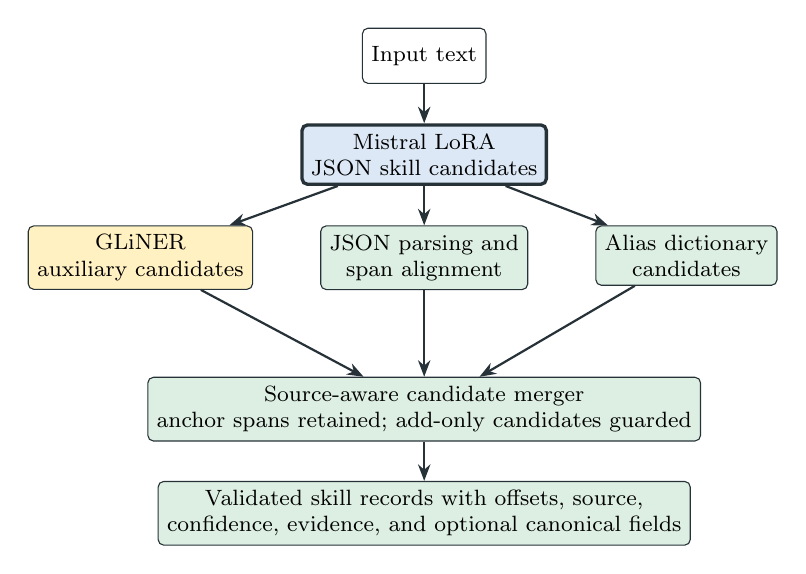
\begin{tikzpicture}[node distance=5mm and 6mm]
\node[data] (text) {Input text};
\node[anchorbox,below=of text] (mistral) {Mistral LoRA\\JSON skill candidates};
\node[exp,below left=of mistral] (gliner) {GLiNER\\auxiliary candidates};
\node[impl,below=of mistral] (align) {JSON parsing and\\span alignment};
\node[impl,below right=of mistral] (dict) {Alias dictionary\\candidates};
\node[impl,below=11mm of align] (merge) {Source-aware candidate merger\\anchor spans retained; add-only candidates guarded};
\node[impl,below=of merge] (skills) {Validated skill records with offsets, source,\\confidence, evidence, and optional canonical fields};
\draw[flow] (text)--(mistral); \draw[flow] (mistral)--(align);
\draw[flow] (mistral)--(gliner); \draw[flow] (mistral)--(dict);
\draw[flow] (align)--(merge); \draw[flow] (gliner)--(merge); \draw[flow] (dict)--(merge); \draw[flow] (merge)--(skills);
\end{tikzpicture}

\caption{Implemented extraction path. The anchor creates source-grounded candidates; GLiNER and dictionary components can add candidates but do not replace the anchor by default.}
\label{fig:extraction}
\end{figure}

\section{Auxiliary extraction, merging, and refinement}

GLiNER and the dictionary extractor have different roles. GLiNER can propose labels from a generalist NER model, while the dictionary extractor looks for aliases in taxonomy files and supports exact/fuzzy matching. Neither source is treated as automatically correct. \inlinecode{CandidateMerger} first validates every candidate, groups surface forms by normalised/alias-equivalent key and label, retains source provenance in \inlinecode{metadata.sources}, and removes redundant subsumed candidates. It then applies its add-only policy. An anchor candidate is recognised by a Mistral source; it is kept. A candidate without Mistral provenance must meet a configurable minimum confidence that depends on its source combination, and it may require exact alias evidence. Candidate spans overlapping an anchor span are withheld under the policy.

Boundary refinement, span verification, and confidence calibration are deliberately separate modules. The boundary refiner can preserve an original candidate or produce an annotated edit. Its tests assert that it preserves an unsubstantiated long span and never drops a candidate simply because a refinement is unavailable. The verifier applies deterministic checks and can reject generic material; the calibrator applies source- and label-sensitive thresholds. These are useful guardrails, but the source-level controls are not a substitute for empirical generalization. The attached span-verifier artifact shows that a model/dataset path exists, while the audit does not find a comprehensive learned-verifier outcome evaluation to report.

\section{Safe-wrapper selection}

The safe-wrapper entry point starts from cached 80-epoch Mistral predictions for the same 974-document evaluation path. It creates three variants: boundary refinement, Mistral plus GLiNER plus taxonomy, and a full path with merger, refiner, verifier, calibrator, and taxonomy linker. The non-regression gate then evaluates each candidate against anchor metrics and selects the candidate predictions only if exact-span and soft-skill floors are met. If either guardrail fails, the selected extraction predictions are the untouched anchor predictions even though linked candidates can still be produced for downstream inspection.

\begin{figure}[H]
\centering
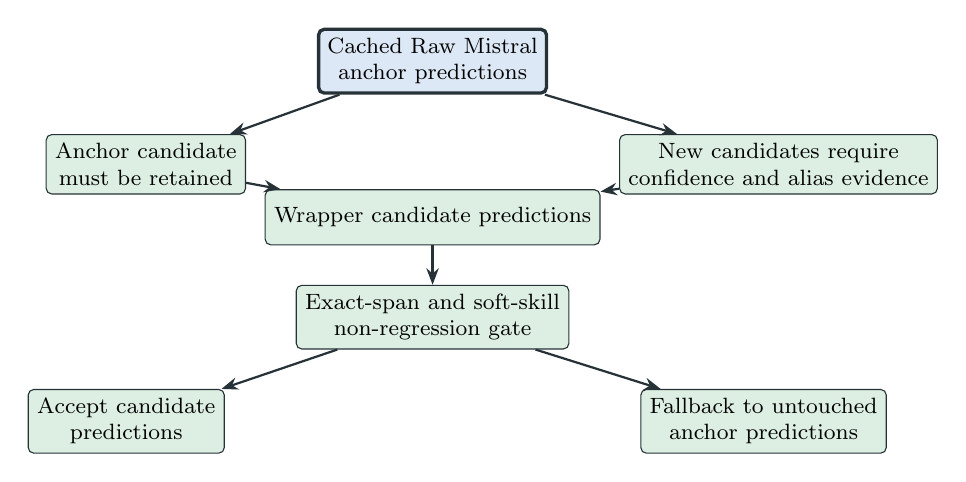
\begin{tikzpicture}[node distance=5mm and 9mm]
\node[anchorbox] (anchor) {Cached Raw Mistral\\anchor predictions};
\node[impl,below left=of anchor] (protect) {Anchor candidate\\must be retained};
\node[impl,below right=of anchor] (add) {New candidates require\\confidence and alias evidence};
\node[impl,below=12mm of anchor] (candidate) {Wrapper candidate predictions};
\node[impl,below=of candidate] (gate) {Exact-span and soft-skill\\non-regression gate};
\node[impl,below left=of gate] (accept) {Accept candidate\\predictions};
\node[impl,below right=of gate] (fallback) {Fallback to untouched\\anchor predictions};
\draw[flow] (anchor)--(protect); \draw[flow] (anchor)--(add); \draw[flow] (protect)--(candidate); \draw[flow] (add)--(candidate); \draw[flow] (candidate)--(gate); \draw[flow] (gate)--(accept); \draw[flow] (gate)--(fallback);
\end{tikzpicture}

\caption{Safe-wrapper design. Protection occurs twice: candidate merging preserves Mistral-originated spans, and the evaluation gate can fall back to cached anchor predictions.}
\label{fig:safe-wrapper}
\end{figure}

The gate is an output-selection mechanism, not a proof of causal improvement. In the persisted safe-wrapper artifact, all three variants receive \inlinecode{accept}, but their \inlinecode{improved_over_anchor} fields are false because none reaches the historical target of 0.675034 exact F1. This is a valuable distinction for a system report. A quality floor can be a reasonable deployment safeguard, while an improvement claim needs stronger evidence such as repeated paired runs, confidence intervals, or a pre-registered evaluation protocol.

\section{Canonicalization and taxonomy attachment}

\inlinecode{TaxonomyLinker} turns a surface form into an optional canonical identifier and name. The alias infrastructure builds an index from configured records; the analysis report identifies 696 canonical entries in the current table. The linker can record alias, fuzzy, and BM25-like decisions. Its essential architectural rule is attach-only behaviour: re-linking never changes \inlinecode{surface_form}, \inlinecode{start}, \inlinecode{end}, \inlinecode{label}, or \inlinecode{source}. This makes canonicalization orthogonal to extraction scoring. A later matching layer may use the canonical ID, but an evaluator can always recover the original text and source.

\begin{figure}[H]
\centering
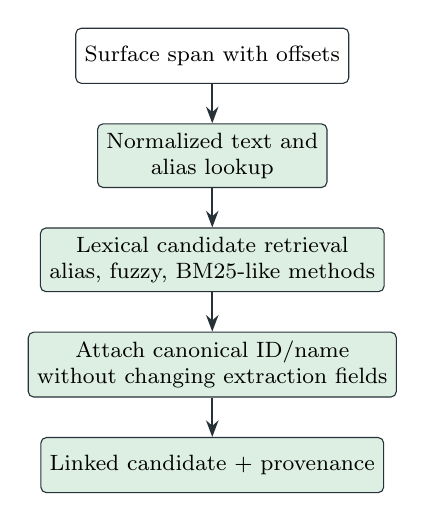
\begin{tikzpicture}[node distance=5mm]
\node[data] (surface) {Surface span with offsets};
\node[impl,below=of surface] (alias) {Normalized text and\\alias lookup};
\node[impl,below=of alias] (retrieve) {Lexical candidate retrieval\\alias, fuzzy, BM25-like methods};
\node[impl,below=of retrieve] (attach) {Attach canonical ID/name\\without changing extraction fields};
\node[impl,below=of attach] (record) {Linked candidate + provenance};
\draw[flow] (surface)--(alias); \draw[flow] (alias)--(retrieve); \draw[flow] (retrieve)--(attach); \draw[flow] (attach)--(record);
\end{tikzpicture}

\caption{Attach-only normalization. The canonical fields enrich a candidate but do not rewrite the extraction fields used by span evaluation.}
\label{fig:normalization}
\end{figure}

The implementation includes loaders named for ESCO, O*NET, Lightcast, and custom records. The reported configuration points at local custom aliases. It is therefore precise to call this an extensible taxonomy interface with a local alias-backed evaluation path. It is imprecise to call it a complete production import of every external taxonomy. The distinction is reinforced by the linking reports: high coverage is available, but a gold canonical-ID dataset for accuracy is not.

\section{Context, graph, and downstream services}

The \inlinecode{context} package transforms already extracted skills into a \inlinecode{ProfileSummary}. Each skill fact carries a surface form, hard/soft label, optional canonical fields, maximum confidence, a list of evidence items, and source offsets. Grouping uses a canonical identifier where present and normalised surface form otherwise. When labels conflict, the summary writes a conflict note. It neither infers a hidden capability nor resolves a contradiction through an opaque model. \inlinecode{SkillMemory} groups facts by label and constructs an alias index. The cached-context builder serialises a packet and stores a SHA-256 content hash, enabling a direct equality check for identical inputs.

The graph layer uses \inlinecode{networkx.MultiDiGraph}. It has typed User, Profile, Job, Course, Skill, SkillCluster, and Occupation nodes. Its direct retrieval functions list a user's skills, a job's required skills, and courses that teach a skill; the explainer attempts a shortest path. The \inlinecode{JobMatcher}, \inlinecode{GapDetector}, and \inlinecode{CourseRecommender} consume simple dictionaries and expose their components in output records. This creates a transparent vertical slice from extracted spans to recommendations, but it is intentionally not presented as a deployed service, learned retriever, or empirically validated career adviser.

\begin{figure}[H]
\centering
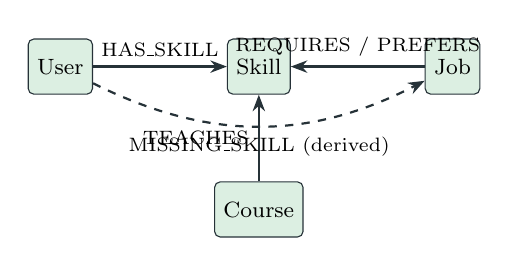
\begin{tikzpicture}[node distance=11mm and 17mm]
\node[impl] (user) {User};
\node[impl,right=of user] (skill) {Skill};
\node[impl,right=of skill] (job) {Job};
\node[impl,below=of skill] (course) {Course};
\draw[flow] (user)--node[above,font=\scriptsize]{HAS\_SKILL}(skill);
\draw[flow] (job)--node[above,font=\scriptsize]{REQUIRES / PREFERS}(skill);
\draw[flow] (course)--node[left,font=\scriptsize]{TEACHES}(skill);
\draw[dashedflow] (user) to[bend right=27] node[below,font=\scriptsize]{MISSING\_SKILL (derived)} (job);
\end{tikzpicture}

\caption{Implemented in-memory knowledge-graph schema. A missing skill is derived from a user/job comparison; it is not an asserted source fact.}
\label{fig:graph}
\end{figure}

\section{Architecture summary}

The completed architecture has one authoritative extraction record and multiple carefully constrained enrichments. At no point does the diagram require an unverified model to overwrite a source span. This makes the system suitable for iterative research: new linkers, retrievers, graph stores, or learned rankers can be introduced behind stable record contracts and evaluated separately. The same modularity also exposes the current boundary: only the extraction and wrapper metrics have full-test numeric evidence; the rest of the architecture must be judged as implemented design and smoke-tested data flow until labelled downstream evaluation is added.

\chapter{Dataset and Experimental Methodology}
\label{ch:methodology}

\section{Evidence-first methodology}

The methodology follows a strict evidence hierarchy. A quantitative statement in this report must come from a persisted metric artifact, a generated report derived from such an artifact, a configuration file, a training summary, or a local data file. A source module establishes that an interface or algorithm is implemented, but it does not establish its performance. A status marker establishes that an automated stage finished, but it does not establish that the result is a full-scale experiment. This hierarchy is necessary because the repository contains full-test outputs, smoke tests, demo records, historical analyses, and an initially uncommitted working tree.

The audit written before this report is the operational version of this method. It reconciles the later safe-wrapper artifacts with an earlier wrapper-error report, identifies the primary result files, and records unavailable downstream metrics as `NA`. The result is more conservative than treating every number found in the directory as interchangeable, but it makes the final argument reproducible and falsifiable.

\section{Dataset and local representation}

The primary corpus is the local export at \codepath{data/source/skillspan\_hf}. Its README attributes SkillSpan to Zhang et al.~\cite{zhang2022skillspan}, specifies CC BY 4.0 licensing, and identifies the English job-posting sources as StackOverflow/technical and STAR/house. Each JSON line has an \inlinecode{idx} document delimiter, token list, \inlinecode{tags_skill}, \inlinecode{tags_knowledge}, and source. The tag names should not be equated mechanically with the report's hard/soft labels without inspecting the data-preparation path; the project creates its internal typed span representation from the local export.

\begin{table}[H]
\centering
\caption{Local SkillSpan export used by the Stage-2 pipeline. The local JSON line counts match the dataset README.}
\label{tab:dataset-splits}
\begin{tabular}{lrp{0.50\textwidth}}
\toprule
Split & Sentences & Use in this report \\
\midrule
Train & 4,800 & Supervised fine-tuning examples \\
Development & 3,174 & Persisted training evaluation and development split \\
Test & 3,569 & Local corpus test partition; the reported cached Mistral evaluation path contains 974 documents \\
\bottomrule
\end{tabular}
\end{table}


The total local row count is 11,543. This is smaller than a naive reading of the paper's 14.5K sentence description only if one mistakes rows or pre-processing states for the original corpus. The thesis reports both facts as separate: the original paper's corpus description and the actual local split counts consumed by this pipeline. It does not invent a reconciliation that is absent from repository artifacts.

\section{SFT data preparation and prompt contract}

\inlinecode{build_mistral_sft_data.py} iterates over train, development, and test splits and writes a JSONL record with four elements: an identifier, an instruction, original input text, and an output object holding gold skills. The training renderer then produces a Mistral chat sequence consisting of a system instruction, a user request containing the source text, and an assistant JSON target. The target strips offsets and retains text plus label. At evaluation time, offsets are re-established by source-string alignment. This choice is significant: training teaches structured string production, whereas evaluation insists that the predicted string maps back to an observed substring.

The prompt requests only explicit mentions and asks for JSON with a \inlinecode{skills} array containing \inlinecode{text} and \inlinecode{label} values. It permits hard, soft, and generic \inlinecode{SKILL} labels at the interface, with generic values mapped to hard skill in the extractor. No free-form explanation is requested from the model, which narrows the decoding surface and makes parse errors observable. The prompt can reduce certain formatting failures; it does not guarantee schema adherence or semantic correctness. The parser and validator remain necessary.

\section{Training procedure}

The full configuration is \codepath{configs/skillllm\_v2\_training\_80ep\_2gpu.yaml}. It specifies seed 42 and an 80-epoch full run. \inlinecode{mistral_lora_trainer.py} loads the model locally, selects bfloat16 when supported and float16 otherwise, configures 4-bit NF4 loading when enabled, prepares the model for k-bit training, enables gradient checkpointing, and injects LoRA adapters into the listed projection modules. The trainer uses a causal language-model objective over rendered chat text, a cosine scheduler, 5\% warmup by default, an 8-bit paged AdamW optimizer in the 4-bit path, and no external reporting backend.

\begin{table}[H]
\centering
\caption{Verified Mistral LoRA settings from \codepath{skillllm\_v2\_training\_80ep\_2gpu.yaml} and the persisted training summary.}
\label{tab:training-config}
\begin{tabular}{ll}
\toprule
Setting & Value \\
\midrule
Seed & 42 \\
Backbone & Mistral Small 3.1 24B Instruct \\
Adaptation & LoRA; rank 16, alpha 32, dropout 0.05 \\
Quantization & 4-bit loading; NF4 path in source \\
Epochs & 80 \\
Batch / accumulation & 1 / 32 \\
Learning rate & 0.00012 \\
Maximum sequence length & 512 \\
Parallelism & 2-process DDP, GPUs 0 and 1 \\
Recorded runtime & 324,217.825 seconds \\
\bottomrule
\end{tabular}
\end{table}


The persisted training summary records a two-process world size, 4,800 training samples, 3,174 development samples, epoch 80, a training loss of 0.143082, a development loss of 0.397449, and 324,217.825 seconds of training runtime. The research-refresh manifest records two RTX 3090 GPUs, PyTorch 2.6.0+cu124, and Python 3.12.3. These records make the compute account concrete. They do not make loss directly comparable with other projects, prove that the final epoch is globally optimal, or quantify seed sensitivity.

\begin{figure}[H]
\centering
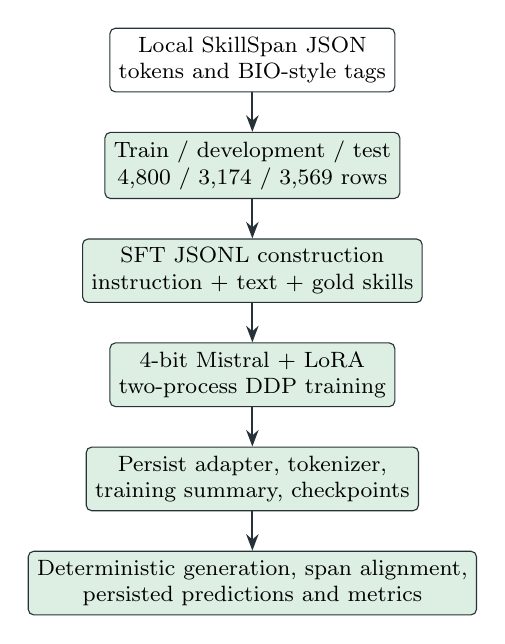
\begin{tikzpicture}[node distance=5mm]
\node[data] (skillspan) {Local SkillSpan JSON\\tokens and BIO-style tags};
\node[impl,below=of skillspan] (splits) {Train / development / test\\4,800 / 3,174 / 3,569 rows};
\node[impl,below=of splits] (sft) {SFT JSONL construction\\instruction + text + gold skills};
\node[impl,below=of sft] (train) {4-bit Mistral + LoRA\\two-process DDP training};
\node[impl,below=of train] (adapter) {Persist adapter, tokenizer,\\training summary, checkpoints};
\node[impl,below=of adapter] (eval) {Deterministic generation, span alignment,\\persisted predictions and metrics};
\draw[flow] (skillspan)--(splits); \draw[flow] (splits)--(sft); \draw[flow] (sft)--(train); \draw[flow] (train)--(adapter); \draw[flow] (adapter)--(eval);
\end{tikzpicture}

\caption{Training and evaluation pipeline traced to the local data-preparation and trainer modules. The persisted evaluation artifact is distinct from smoke-mode fallback.}
\label{fig:training}
\end{figure}

\section{Baselines and comparison discipline}

The project contains a BERT baseline and a GLiNER baseline. The BERT metric file identifies itself as a CPU-fast token-classification baseline. The GLiNER metric file states that fine-tuning was skipped and that the run is zero-shot/few-shot. Both are useful reference points because they use the same local evaluation tooling and show the magnitude of the Mistral result in the repository. They are not intended as exhaustive tuned baselines. In particular, their lower results cannot support a general conclusion that all encoder models or all generalist NER systems are ineffective for skill extraction.

The report also distinguishes legacy Phase-A and Stage-2 evidence. A root-level thesis evidence report references earlier multi-LLM benchmarks with different epoch counts and configurations. They have research value, but the present numeric comparison table is restricted to Stage-2 persisted artifacts. This avoids combining a three-epoch result, a 80-epoch result, a smoke test, and a demo under one apparent benchmark protocol.

\section{Extraction evaluation}

The extraction evaluator compares gold and predicted spans and reports exact span, partial span, token, hard-skill, soft-skill, macro, and micro metrics. Exact matching uses label and boundary agreement. Partial matching and token F1 provide diagnostic context when a system locates a relevant phrase but selects a different boundary. The primary metric is exact-span F1 because downstream canonicalization is only meaningful when it can be traced to a source span. Parse failure and alignment information further distinguish a model that has no candidate from one that emits ungrounded text.

For wrapper experiments, the methodology is paired: cached anchor predictions and candidate wrapper predictions are evaluated on the same 974-document path. The safe-wrapper script records candidate and selected metrics, guardrail floors, deltas, a decision, and an explanation. This is stronger than comparing unrelated aggregate runs, yet still not a multi-seed statistical study. It identifies whether a particular wrapper snapshot is compatible with the anchor; it does not estimate a population-level treatment effect.

\begin{figure}[H]
\centering
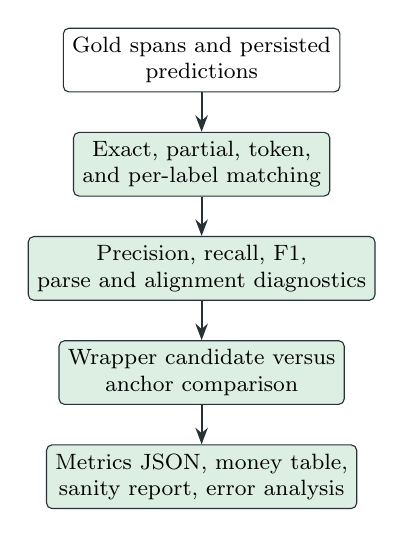
\begin{tikzpicture}[node distance=5mm]
\node[data] (gold) {Gold spans and persisted\\predictions};
\node[impl,below=of gold] (align) {Exact, partial, token,\\and per-label matching};
\node[impl,below=of align] (metrics) {Precision, recall, F1,\\parse and alignment diagnostics};
\node[impl,below=of metrics] (wrapper) {Wrapper candidate versus\\anchor comparison};
\node[impl,below=of wrapper] (report) {Metrics JSON, money table,\\sanity report, error analysis};
\draw[flow] (gold)--(align); \draw[flow] (align)--(metrics); \draw[flow] (metrics)--(wrapper); \draw[flow] (wrapper)--(report);
\end{tikzpicture}

\caption{Evaluation path for extraction and wrapper selection. Downstream ranking metrics use a separate, currently unavailable labelled protocol.}
\label{fig:evaluation}
\end{figure}

\section{Normalization and downstream methodology}

Linking evaluation is deliberately separated from extraction. The taxonomy error-analysis report evaluates how often candidate records obtain canonical attachments from a 696-entry local alias table and breaks methods down into BM25, alias, fuzzy, and none. Because no gold canonical IDs are supplied for a supervised reranker, the reported 0.890 values are coverage measures. The \inlinecode{linking_eval.csv} file has \inlinecode{taxonomy_linking_accuracy,0.0}; it must not be overwritten with coverage in a final table.

The graph, job matching, gap detection, and course recommendation modules are exercised through unit tests and demo artifacts. Their output formats include matched skills, missing skills, evidence strings, recommendation reasons, and courses that cover gaps. Neither \inlinecode{matching_eval.csv} nor \inlinecode{course_recommendation_eval.csv} has a usable label-derived score: nDCG@10 and P@5 are both `NA`. Accordingly, this report analyses their data flow and formulas, not their real-world efficacy.

\section{Reproducibility procedure}

The implementation produces a layered trail: configuration leads to adapter/checkpoint and training-summary artifacts; generation leads to predictions, raw outputs, and metrics; wrapper processing leads to candidate and linked records; reports summarise the results. \inlinecode{prediction_provenance_check.py} verifies that selected downstream files are newer than the upstream Mistral predictions and rejects a metric note indicating fallback use. The report states that no stale or missing downstream artifacts were detected. Timestamps are useful safeguards but are not a replacement for versioned Git history, immutable artifact storage, checksums of every input, or environment lock files. Those items are future reproducibility work.

\chapter{Experiments}
\label{ch:experiments}

\section{Experimental objectives}

The experiments are organised around a narrow claim: identify the strongest extraction anchor in the persisted Stage-2 artifacts and test whether modular additions remain compatible with it. This differs from a broad model sweep. The repository contains earlier multi-model work, but the current Stage-2 study is Mistral-focused and uses stored artifacts from an 80-epoch training path. The comparisons answer three practical questions. First, can the adapted causal model produce source-aligned hard and soft skill spans substantially better than the included BERT and zero-shot GLiNER reference artifacts? Second, do boundary, auxiliary-candidate, taxonomy, and full-wrapper paths alter the anchor metrics? Third, are the resulting records usable by the implemented profile, graph, matching, and recommendation paths without converting smoke success into a ranking claim?

All reported numeric comparisons are descriptive measurements from the persisted files. The work does not report confidence intervals, significance tests, or multi-seed variation because those artifacts are absent. A difference smaller than a thousandth should be read as an observation in this evaluation snapshot, not as a robust superiority statement.

\section{Experiment E1: extraction baselines}

E1 compares the BERT baseline, GLiNER baseline, and Raw Mistral LoRA anchor. The BERT file reports exact-span F1 0.059150, token F1 0.274922, hard-skill F1 0.129799, and soft-skill F1 0.018796. Its note calls it a CPU-fast token-classification baseline. The GLiNER file reports exact-span F1 0.075833, token F1 0.114409, hard-skill F1 0.054559, and soft-skill F1 0.096571. It explicitly identifies the run as zero-shot because fine-tuning was skipped. These labels constrain interpretation: E1 compares available local reference implementations, not fully optimized replications of the BERT or GLiNER literature.

The Mistral anchor was trained with the settings in \Cref{tab:training-config}. Its result is evaluated through deterministic JSON generation, parsing, substring alignment, and the extraction evaluator. Its artifact says `Model load fallback used: False`, which is a crucial validity condition because the extractor contains a deterministic smoke fallback for unavailable model files. The Mistral value is therefore the main model result in this report.

\section{Experiment E2: historical wrapper diagnosis}

E2 is a historical diagnostic, not a row in the primary result table. \inlinecode{wrapper_error_analysis.md} reports an anchor of 0.675034 exact F1 and 0.609792 soft F1 on a 974-document test path. It reports that an older boundary-refiner variant fell to approximately 0.5704 exact F1 and 0.4258 soft F1, while an older full CAG/graph path fell to approximately 0.5616 exact F1 and 0.4080 soft F1. The diagnosis attributes 194 boundary-related regressions to the boundary refiner in the full path and 29 further cases to verifier false rejection. It is a valuable negative result: a post-processor can reduce a model's exactness even when its stated purpose is to clean up spans.

The audit found later full-test artifacts created after this analysis. Their anchor has 0.670069 exact F1 rather than 0.675034, and their safe-wrapper code uses anchor-protection and a gate. These runs should not be averaged or represented as a single ablation series. E2 explains the engineering response; E3 provides the current metric snapshot.

\section{Experiment E3: safe-wrapper variants}

E3 loads the cached full-test Mistral predictions and evaluates three wrapper variants on the same document path. The first applies a non-destructive boundary refiner with verifier and calibrator. The second combines Mistral, GLiNER, and dictionary candidates, applies an anchor-protected merger, then attaches taxonomy information. The third combines the merger, boundary refiner, verifier, calibrator, and taxonomy linker in the full CAG/graph path. The script writes both candidate predictions and selected predictions so that a fallback decision is inspectable.

The active guardrails compare exact-span and soft-skill metrics with the anchor. A candidate can be accepted while still failing to reach the historical improvement target. This is intentional. The policy defines a deployment-like safety threshold, whereas the improvement target remains an informational goal. In the stored output, all variants are accepted because each clears exact and soft floors. The Mistral+GLiNER+taxonomy candidate is 0.000007 lower in exact F1 and 0.001741 lower in soft F1 than the anchor; the full candidate is 0.001033 higher in exact F1 but 0.000291 lower in soft F1. Such deltas should be treated as essentially a compatibility result, not a reason to prefer one architecture on accuracy alone.

\begin{table}[H]
\centering
\small
\caption{Safe-wrapper gate results. Acceptance means that the candidate clears configured non-regression floors; it does not mean that it reached the historical improvement target.}
\label{tab:gate-results}
\begin{tabular}{lrrrrl}
\toprule
Variant & Anchor exact & Candidate exact & Anchor soft & Candidate soft & Decision \\
\midrule
Boundary refiner & 0.670069 & 0.671111 & 0.604046 & 0.605505 & accept \\
GLiNER + taxonomy & 0.670069 & 0.670062 & 0.604046 & 0.602305 & accept \\
Full CAG/graph & 0.670069 & 0.671102 & 0.604046 & 0.603755 & accept \\
\bottomrule
\end{tabular}
\end{table}


\section{Experiment E4: taxonomy attachment}

E4 evaluates whether the local linker attaches canonical fields to wrapper candidates. The analysis report states that an earlier four-entry fallback was replaced by a 696-entry alias table. For the Mistral+GLiNER+taxonomy path, it reports total linking coverage 0.882139 under a detailed analysis and 0.890271 in the metric artifact; for the full path it reports 0.838908 in the detailed analysis and 0.890374 in the metric artifact. These values reflect different candidate artifacts/stages and should not be collapsed. The primary table uses the metric-artifact value, while the detailed report remains useful for error categories and unlinked surface forms.

Most importantly, no canonical gold labels are available for a supervised reranker. The project reports method counts for alias, fuzzy, BM25, and no link, but cannot establish that every attachment is correct. E4 therefore supports an engineering claim---the normalizer attaches canonical metadata with broad local coverage---not a semantic-accuracy claim. The attach-only constraint ensures that a wrong link does not alter the original span metrics, though it can still harm a downstream recommendation and must be evaluated later.

\section{Experiment E5: profile, graph, and recommendation vertical slice}

E5 is an integration and smoke experiment. The profile summarizer aggregates extracted skills, their evidence, and their offsets. The cached-context builder separates stable profile memory, dynamic job-posting retrieval policy, and graph-path policy, then computes a content hash. The graph builder creates typed nodes and direct relationships; the matcher, gap detector, and recommender emit inspectable JSON objects. Unit tests verify a representative user--skill--job--course flow, and demo artifacts contain a profile, job matches, skill gaps, course recommendations, and an explanation.

The evidence supports a vertical-slice claim: records can travel from extraction into a structured profile and then into explainable downstream objects. It does not support a utility claim. The matching-evaluation CSV records job nDCG@10 as `NA`, and the course-recommendation evaluation CSV records P@5 as `NA`, because relevance labels are unavailable. No human-subject study, click-through test, or offline ranking benchmark is stored. Thus E5 evaluates execution and traceability, not recommendation quality.

\section{Artifact tracking and protocol fidelity}

\Cref{fig:provenance} shows the experimental artifact path. The project writes model-training summaries, model files, predictions, raw outputs, metrics, gate reports, money tables, and error analyses under conventional artifact/report directories. The provenance-check script compares downstream modification times with Mistral predictions and checks the metrics note for fallback use. The persisted report indicates no stale or missing artifacts. This check prevents a common research-reporting failure in which a downstream table is silently generated from an older anchor output.

\begin{figure}[H]
\centering
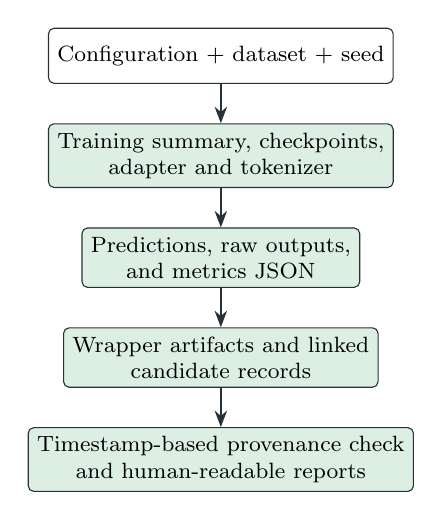
\begin{tikzpicture}[node distance=5mm]
\node[data] (config) {Configuration + dataset + seed};
\node[impl,below=of config] (train) {Training summary, checkpoints,\\adapter and tokenizer};
\node[impl,below=of train] (pred) {Predictions, raw outputs,\\and metrics JSON};
\node[impl,below=of pred] (down) {Wrapper artifacts and linked\\candidate records};
\node[impl,below=of down] (check) {Timestamp-based provenance check\\and human-readable reports};
\draw[flow] (config)--(train); \draw[flow] (train)--(pred); \draw[flow] (pred)--(down); \draw[flow] (down)--(check);
\end{tikzpicture}

\caption{Artifact and provenance pipeline. The timestamp check is a practical safeguard, not an immutable experiment-management system.}
\label{fig:provenance}
\end{figure}

The remaining protocol limits are clear. The Stage-2 tree has no commit, a model-selection criterion beyond the stored output is not documented as a pre-registration, the full evaluation path contains 974 documents despite the local test JSON having 3,569 rows, and multi-seed reruns are absent. Future experiments should version every source and configuration, explain the 974-document evaluation subset in a machine-readable manifest, and predefine their primary score and selection rule.

\chapter{Results}
\label{ch:results}

\section{Primary extraction results}

\Cref{tab:main-results} presents the thesis's primary numerical result table. It is generated from the persisted Stage-2 metric artifacts and agrees with the metric-sanity and money-table reports. The Raw Mistral LoRA path is the clear anchor within this collection: exact-span F1 is 0.670069, token F1 0.787886, hard-skill F1 0.726450, and soft-skill F1 0.604046. The result is substantially larger than the stored BERT and zero-shot GLiNER scores. The appropriate conclusion is local and bounded: under this repository's stored evaluator, training path, and artifact set, the adapted Mistral extractor is the best available extraction component.

\begin{table}[H]
\centering
\small
\caption{Primary full-test extraction artifacts. Values are copied from persisted \codepath{metrics.json} files, not inferred from prose reports.}
\label{tab:main-results}
\begin{tabular}{lrrrr}
\toprule
System & Exact F1 & Token F1 & Hard F1 & Soft F1 \\
\midrule
BERT baseline & 0.059150 & 0.274922 & 0.129799 & 0.018796 \\
GLiNER baseline (zero-shot) & 0.075833 & 0.114409 & 0.054559 & 0.096571 \\
Raw Mistral LoRA anchor & 0.670069 & 0.787886 & 0.726450 & 0.604046 \\
Mistral + GLiNER + taxonomy & 0.670062 & 0.787575 & 0.728020 & 0.602305 \\
Full CAG/graph wrapper & 0.671102 & 0.787575 & 0.728618 & 0.603755 \\
\bottomrule
\end{tabular}
\end{table}


The contrast between exact and token F1 is informative. For the Mistral anchor, token F1 exceeds exact F1 by about 0.118. This pattern is expected when some predicted regions overlap gold spans but have non-identical boundaries. It reinforces why a report on a downstream career system must not use a token-only measure: the original surface span is later used for evidence display and canonicalization. The hard/soft difference is also material. Soft-skill F1 is about 0.122 lower than hard-skill F1 for the anchor, leaving a clear target for future annotation analysis and model improvement.

The BERT and GLiNER measurements should not be misread as a literature leaderboard. BERT is identified as a CPU-fast baseline, and GLiNER is zero-shot/few-shot. Nonetheless, they are useful controls because they reveal that the result is not a minor score variation around a shared baseline. They also illustrate a methodological lesson: merely inserting a general NER component does not establish suitability for typed skill spans under an exact evaluation interface.

\begin{figure}[H]
\centering
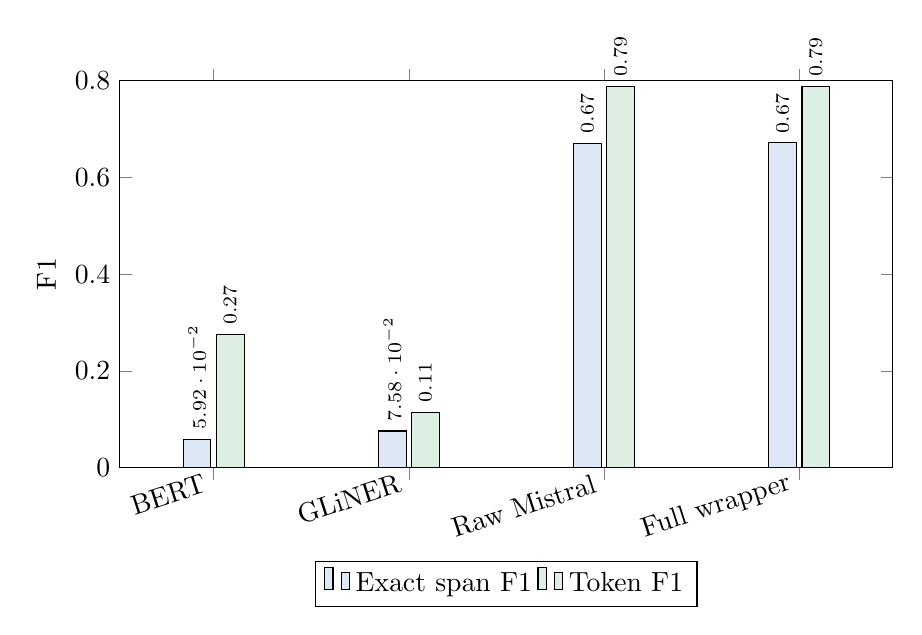
\begin{tikzpicture}
\begin{axis}[
  ybar,bar width=10pt,width=0.94\textwidth,height=6.5cm,
  ymin=0,ymax=0.8,ylabel={F1},
  symbolic x coords={BERT,GLiNER,Raw Mistral,Full wrapper},
  xtick=data,xticklabel style={rotate=18,anchor=east},
  legend style={at={(0.5,-0.24)},anchor=north,legend columns=2},
  nodes near coords, every node near coord/.append style={font=\scriptsize,rotate=90,anchor=west},
  enlarge x limits=0.16]
\addplot[fill=anchor] coordinates {(BERT,0.059150) (GLiNER,0.075833) (Raw Mistral,0.670069) (Full wrapper,0.671102)};
\addplot[fill=implemented] coordinates {(BERT,0.274922) (GLiNER,0.114409) (Raw Mistral,0.787886) (Full wrapper,0.787575)};
\legend{Exact span F1,Token F1}
\end{axis}
\end{tikzpicture}

\caption{Exact-span and token F1 from primary persisted artifacts. The full wrapper's exact-span difference from Raw Mistral is 0.001033 and should not be interpreted as a robust gain.}
\label{fig:results-chart}
\end{figure}

\section{Wrapper results and selection semantics}

The wrapper variants preserve the headline result rather than transform it. The boundary-safe variant records 0.671111 exact F1 and 0.605505 soft F1. The Mistral+GLiNER+taxonomy variant records 0.670062 and 0.602305. The full CAG/graph variant records 0.671102 and 0.603755. Each selected result passes the gate's configured floors, and each is marked `accept`. The full wrapper has the largest exact F1 observed among these files, but its advantage over the Mistral anchor is only 0.001033. Its soft-skill F1 is slightly lower than the anchor's. The evidence supports the wording ``accepted as non-regressive under configured tolerances''; it does not support ``wrapper improves extraction.''

This result is scientifically useful rather than disappointing. It means that a modular pipeline can enrich extraction with source, canonicalization, context, and graph metadata without a large measured loss in the stored evaluation. It also warns against using wrapper complexity as a substitute for a strong primary model. A consumer of the output can treat Mistral as the provenance source for extraction and treat the wrapper as a guarded enrichment layer. The architecture remains valuable even in the absence of a large F1 increase because downstream systems need IDs, evidence, and explanations, but their value must be evaluated on their own metrics.

\section{Linking and downstream results}

The full CAG/graph metrics file records \inlinecode{linking_accuracy} 0.890374, while the detailed linking report calls the same kind of quantity coverage and states that supervised reranker labels are unavailable. The safer term is therefore \emph{linking coverage}: a large share of candidate records obtained a canonical attachment from the local alias system. It cannot be called canonical-link accuracy without a gold target. The code's attach-only property protects extraction F1 from the addition of a canonical field, but it does not establish the correctness of all attached IDs.

The downstream result status is even more constrained. The full wrapper's metric file contains null values for job nDCG@10 and course precision@5, and their report CSV files write `NA`. The code produces job-match scores, gap types, recommended courses, and explanations. The integration slice is therefore available for qualitative inspection and future annotation, but no quantitative claim is made about relevance, fairness, usefulness, or hiring outcomes.

\section{Answer to the research questions}

RQ1 is answered by the Mistral artifact: the primary model obtains 0.670069 exact-span F1 and 0.604046 soft-skill F1 in the stored Stage-2 evaluation. RQ2 is answered descriptively: the stored BERT and GLiNER baselines are much lower, and the wrapper variants remain near the anchor rather than delivering a large improvement. RQ3 is answered by the code and gate artifacts: candidate source protection, add-only admission, attach-only linking, and fallback are concrete mechanisms that prevent uncontrolled post-processing.

RQ4 is answered at implementation level. The profile/context path preserves extraction evidence and offsets, handles duplicate keys, writes conflicts, separates stable and dynamic context, and hashes a cached packet. RQ5 is answered by an explicit boundary: typed graph, matching, gap, and course modules exist and are smoke-tested, but no labelled nDCG or P@5 evaluation is available. The most important result is therefore a systems result: extraction quality is an invariant that the rest of the architecture must preserve, rather than a quantity downstream components can freely trade away for apparent sophistication.

\chapter{Error Analysis and Non-Regressive Design}
\label{ch:error-analysis}

\section{Why an error analysis is necessary}

Aggregate F1 can conceal the mechanism of a regression. A wrapper may improve the appearance of one candidate while removing many correct anchor spans; a taxonomy linker may attach a plausible identifier to a wrong surface form; a verifier may reject uncommon technical terms as generic language. Because SkillLLM\_v2 is meant to support later explanation, the source of a failure matters as much as its score. The repository contains an unusually informative historical wrapper report and a later safe-wrapper evaluation. Read together, they show why the architecture protects anchor spans and records a selection decision.

\section{Historical destructive post-processing}

The historical \inlinecode{wrapper_error_analysis.md} is not merged into the primary metric table, but it is a strong diagnostic. It reports an anchor exact-span F1 of 0.675034, token F1 of 0.797798, hard-skill F1 of 0.731138, and soft-skill F1 of 0.609792. Its older boundary-refiner path reports approximately 0.5704 exact F1 and 0.4258 soft F1; the older full CAG/graph path reports approximately 0.5616 exact F1 and 0.4080 soft F1. The direction is unambiguous in that historical snapshot: the post-processors reduced extraction quality sharply.

The report attributes 194 full-wrapper regressions to bad boundary edits, two to bad label changes, and 29 to verifier false rejection. It records 225 total full-wrapper regressions. The boundary refiner alone had 194 regressions. These counts identify a root cause more useful than a generic statement that ``the wrapper underperformed.'' A high-quality extractor had already produced a boundary that the downstream rule changed incorrectly. The fix is not a more aggressive rule; it is to retain the anchor unless a correction can be justified and to make the correction observable in metadata.

\begin{table}[H]
\centering
\small
\caption{Historical error diagnosis from \codepath{wrapper\_error\_analysis.md}. These values describe a prior wrapper analysis and are not pooled with the newer primary table.}
\label{tab:historical-errors}
\begin{tabular}{lrrrr}
\toprule
Stage & Exact F1 & Soft F1 & Exact gains & Exact losses \\
\midrule
Raw Mistral anchor & 0.675034 & 0.609792 & -- & -- \\
Boundary refiner & 0.5704 & 0.4258 & 53 & 194 \\
Mistral + GLiNER + taxonomy & 0.6515 & 0.5777 & 36 & 0 \\
Full CAG/graph & 0.5616 & 0.4080 & 78 & 225 \\
\bottomrule
\end{tabular}
\end{table}

The apparent zero regressions in the historical Mistral+GLiNER+taxonomy row do not make it a universal winner; its exact and soft values remain below that historical anchor. They instead suggest that additions and edits have distinct risk profiles. Add-only candidate generation can increase recall without deleting a base prediction, while boundary modification and generic rejection can damage previously correct spans. This observation is implementation-specific and requires renewed testing on every code/configuration change.

\section{From diagnosis to control points}

The current code introduces four control points. First, a candidate with Mistral provenance is anchor-protected in `CandidateMerger`. Second, non-anchor candidates must satisfy confidence and optional alias-evidence requirements before they can be added. Third, the boundary-refiner tests explicitly require preservation when taxonomy evidence is absent and prohibit candidate disappearance. Fourth, the non-regression gate evaluates a candidate wrapper output against exact and soft floors and can select cached anchor predictions instead.

These controls address different failure modes. Source protection stops a merger from deleting an anchor candidate before evaluation. Add-only filtering limits false-positive additions. Boundary preservation stops a local rule from turning uncertainty into an edit. The gate protects the final output even when an earlier module changes behaviour. None of these mechanisms proves semantic correctness. They are layered safeguards with traceable failure modes, which is more appropriate than trusting a complex wrapper as a monolith.

\section{Current safe-wrapper interpretation}

The later safe-wrapper run yields a materially different outcome: all three variants clear the chosen non-regression floors. This shows that the corrected path is at least compatible with the persisted anchor under the recorded evaluation. It does not invalidate the historical diagnosis. Rather, the diagnosis motivated a redesign, and the new run is evidence that the redesign avoided the large measured collapses observed earlier. The experiment is still a single stored snapshot. A new model checkpoint, alias table, or boundary rule could cause another regression and should trigger the same paired evaluation.

The report's honest language matters here. Calling the safe wrapper ``non-regressive'' is correct only relative to its configured floors and artifact path. Calling it ``better'' because one exact F1 value is 0.001033 higher would overstate a difference with no repeated runs or uncertainty estimates. Similarly, a wrapper that falls back to the anchor would not be a failed system: it would have exercised the intended safety mechanism and preserved the primary extraction output.

\section{Likely remaining error categories}

Several error categories remain relevant even where a count is not available. First, the model can produce a correct concept with a string that does not occur verbatim, causing an alignment failure. Second, the same surface string can occur more than once; deterministic occurrence selection may attach a prediction to the wrong mention. Third, hard/soft labels can be ambiguous for terms such as collaboration, communication, project management, or domain-specific practices. Fourth, the local alias table can leave emerging technologies, abbreviations, or malformed source text unlinked. The linking report's unlinked examples include technical names and compressed forms such as `k8s`, `yaml`, and `sonarqube`, showing the practical value of coverage analysis.

Finally, downstream errors can originate upstream even when downstream code is deterministic. A false negative extraction becomes a missing skill, which may lower a match score or cause a course to be recommended unnecessarily. A wrong canonical ID can create a false graph edge. An explicit evidence field, source offset, and explanation string allow a user or researcher to trace such a decision back to a candidate record. This is why provenance is not merely documentation: it is a debugging interface.

\section{Error-analysis protocol for future runs}

Future experiments should preserve the current paired structure and extend it. For each candidate wrapper, save anchor predictions, candidate predictions, selected predictions, and a row-level action log. Stratify errors by hard/soft label, source domain, span length, alias availability, parser outcome, and edit type. Add a blind manual sample review so that a score change can be associated with interpretable examples. Most importantly, keep the extraction anchor immutable during wrapper evaluation. If a new primary model is trained, establish its own artifact, then repeat wrapper evaluation from that version rather than reusing earlier thresholds without verification.

\chapter{Context Intelligence: Profiles, Graphs, Matching, and Recommendations}
\label{ch:context}

\section{From a span list to a durable profile}

Span extraction is intentionally local: given a sentence or document, it returns the capability mentions supported by that text. A career-facing system needs an additional representation that can accumulate evidence across a resume, user-confirmed entries, target roles, completed courses, and interactions. Passing every raw input to a model on every request is inefficient and makes contradictions difficult to inspect. Conversely, replacing the history with an opaque summary risks erasing the source of a claim. SkillLLM\_v2 implements a narrow middle ground: a structured, evidence-preserving profile summary.

\inlinecode{ProfileSkillFact} contains a surface form, a hard/soft label, optional canonical identifier and name, a confidence, a list of evidence records, and metadata. Each evidence record contains a source, text, confidence, and timestamp. \inlinecode{summarize_profile} receives a raw profile text and explicitly supplied extraction results; it does not infer a hidden skill. It groups records by canonical identifier if available, otherwise by normalised surface form. When duplicate evidence arrives, it keeps evidence items and takes the maximum confidence rather than silently averaging away conflicting support. Source offsets are preserved in metadata.

This design gives a later UI or LLM concrete answers to questions such as ``Why does the profile contain Python?'' and ``Which input mentioned this skill?'' It also has a modest conflict mechanism. If the same normalised name arrives under different labels, a conflict note is recorded. It does not yet model temporal recency, evidence reliability by source, proficiency levels, or semantic contradiction. For example, it has no first-class representation of a claim that a user stopped using a tool or has only introductory experience. Those are intended future extensions, not current implicit behaviour.

\begin{figure}[H]
\centering
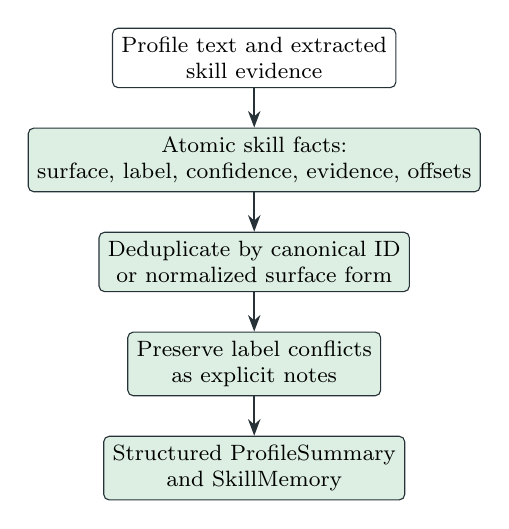
\begin{tikzpicture}[node distance=5mm]
\node[data] (history) {Profile text and extracted\\skill evidence};
\node[impl,below=of history] (facts) {Atomic skill facts:\\surface, label, confidence, evidence, offsets};
\node[impl,below=of facts] (dedupe) {Deduplicate by canonical ID\\or normalized surface form};
\node[impl,below=of dedupe] (conflict) {Preserve label conflicts\\as explicit notes};
\node[impl,below=of conflict] (summary) {Structured ProfileSummary\\and SkillMemory};
\draw[flow] (history)--(facts); \draw[flow] (facts)--(dedupe); \draw[flow] (dedupe)--(conflict); \draw[flow] (conflict)--(summary);
\end{tikzpicture}

\caption{Implemented evidence-preserving profile summarization. It aggregates explicit candidates and records conflicts instead of inferring or silently resolving them.}
\label{fig:profile}
\end{figure}

\section[Context compaction policy]{\hspace{0.35em}Context compaction policy}

The context-compaction function returns three intentionally separate sections. Its stable cache contains a profile summary, skill memory, taxonomy aliases, and optional course-catalog summaries. Its dynamic-retrieval policy identifies job postings and scraped descriptions as sources to retrieve rather than cache. Its graph policy describes user-to-skill-to-job-to-course paths that belong in a relational layer. The cached packet carries the three policies, a packet type, and a SHA-256 hash of the serialised payload.

The terms CAG and RAG are used in this report to describe local context-management roles, not to claim a benchmarked implementation of a particular published CAG/GraphRAG algorithm. The cached portion is stable in the sense of input role, not permanently true; an application must invalidate or recreate it when a user updates their profile. The dynamic policy is a declaration that job records change frequently, not a production web-crawling system. The retrieval class currently performs deterministic lexical overlap over contextualised records. It creates a testable interface but does not claim dense semantic retrieval.

\begin{figure}[H]
\centering
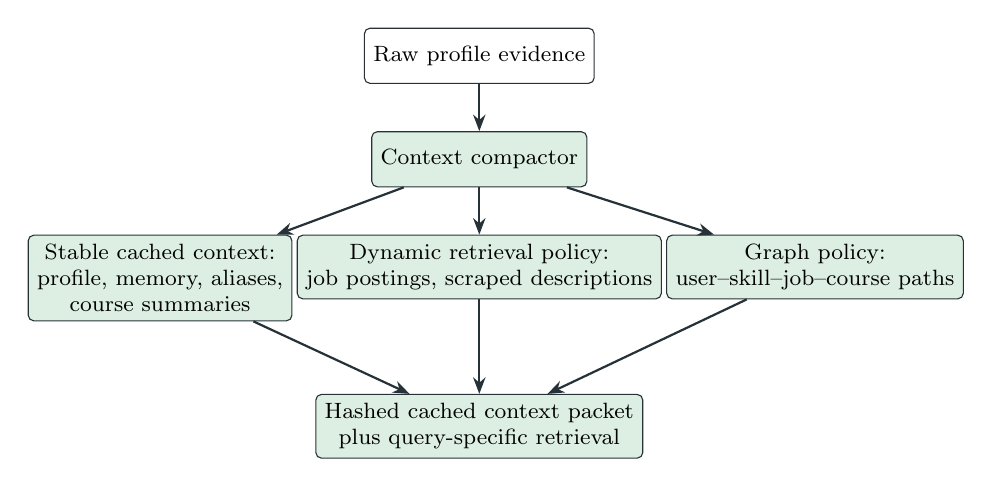
\begin{tikzpicture}[node distance=6mm and 10mm]
\node[data] (raw) {Raw profile evidence};
\node[impl,below=of raw] (compact) {Context compactor};
\node[impl,below left=of compact] (cag) {Stable cached context:\\profile, memory, aliases,\\course summaries};
\node[impl,below=of compact] (rag) {Dynamic retrieval policy:\\job postings, scraped descriptions};
\node[impl,below right=of compact] (graph) {Graph policy:\\user--skill--job--course paths};
\node[impl,below=12mm of rag] (packet) {Hashed cached context packet\\plus query-specific retrieval};
\draw[flow] (raw)--(compact); \draw[flow] (compact)--(cag); \draw[flow] (compact)--(rag); \draw[flow] (compact)--(graph); \draw[flow] (cag)--(packet); \draw[flow] (rag)--(packet); \draw[flow] (graph)--(packet);
\end{tikzpicture}

\caption{Implemented context-compaction policy. Stable profile structures are cached; dynamic job information and graph explanations remain separate responsibilities.}
\label{fig:context-policy}
\end{figure}

\section{Why evidence preservation matters for compaction}

An evidence-preserving compact profile has three system benefits. First, it makes source attribution available after deduplication. A canonical \inlinecode{amazon_web_services} fact can retain both an ``AWS'' resume mention and an ``Amazon Web Services'' job-history mention rather than forcing one surface form to win. Second, it supports constrained updates. A future skill-confidence model can append a new evidence event or revise an aggregation function without rewriting the original extraction. Third, it makes a contextual packet inspectable: the hash detects changes to serialised content, and the separated policy fields reveal why a fact was cached or retrieved.

This approach also reduces a common overclaim in career systems. A user profile is not a ground-truth competency graph merely because it is structured. It is a set of claims with source and confidence. The current profile data type does not determine mastery, duration, recency, or employer validation. A recommendation generated from it should expose that it is based on extracted textual evidence and should invite correction. The existing code's refusal to infer hidden skills is therefore a useful privacy and reliability property.

\section{Knowledge graph representation}

The graph subsystem uses NetworkX to create an in-memory \inlinecode{MultiDiGraph}. It supports User, Profile, Job, Course, Skill, SkillCluster, and Occupation nodes. Its edge vocabulary includes \inlinecode{HAS_SKILL}, \inlinecode{MISSING_SKILL}, \inlinecode{REQUIRES}, \inlinecode{PREFERS}, \inlinecode{TEACHES}, \inlinecode{REQUIRES_PREREQUISITE}, \inlinecode{SIMILAR_TO}, and \inlinecode{BELONGS_TO}. The public builder methods create user-skill, job-requirement, and course-skill relationships. The retriever lists direct neighbours, while the explainer computes a shortest path if one exists and returns a textual arrow-separated explanation.

\begin{figure}[H]
\centering
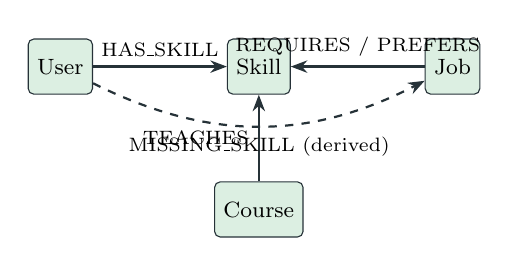
\begin{tikzpicture}[node distance=11mm and 17mm]
\node[impl] (user) {User};
\node[impl,right=of user] (skill) {Skill};
\node[impl,right=of skill] (job) {Job};
\node[impl,below=of skill] (course) {Course};
\draw[flow] (user)--node[above,font=\scriptsize]{HAS\_SKILL}(skill);
\draw[flow] (job)--node[above,font=\scriptsize]{REQUIRES / PREFERS}(skill);
\draw[flow] (course)--node[left,font=\scriptsize]{TEACHES}(skill);
\draw[dashedflow] (user) to[bend right=27] node[below,font=\scriptsize]{MISSING\_SKILL (derived)} (job);
\end{tikzpicture}

\caption{Skill graph relation types used by the current vertical slice. Direct edges are constructed from supplied records; a missing skill is derived.}
\label{fig:graph-schema}
\end{figure}

The graph is useful even before learned graph reasoning. A deterministic graph prevents a downstream explanation from being detached from the skills and course records it used. It allows a path such as user $\rightarrow$ known skill $\rightarrow$ job requirement $\rightarrow$ course to be surfaced for inspection. Still, the present graph does not persist to a database, resolve real-world duplicate entities beyond the linker, learn node embeddings, or evaluate graph retrieval against relevance labels. It should be described as a lightweight graph representation and explanation mechanism.

\section{Job matching and skill-gap detection}

\inlinecode{JobMatcher} consumes a profile with a \inlinecode{skills} list and a job with \inlinecode{required_skills} and \inlinecode{preferred_skills}. It computes overlap, missing required skills, optional supplied semantic-role fit, experience-level fit, user-preference fit, and a penalty proportional to missing required skills. The fixed equation in \Cref{eq:match} is implemented directly in source. The returned record includes a clipped score, matched skills, missing skills, critical missing skills, evidence strings showing coverage, and a short recommendation reason.

\inlinecode{GapDetector} expands the missing-skill view. For a job requirement, a skill can be missing-critical, weak, outdated, uncertain, or covered by an explicitly supplied transferable mapping. Preferred but absent skills form a separate missing-preferred category. This vocabulary is useful for transparency because an absent string and a low-confidence/obsolete skill are not the same intervention. Yet the classification depends on supplied profile fields; the system does not currently estimate proficiency or obsolescence from raw text.

\begin{figure}[H]
\centering
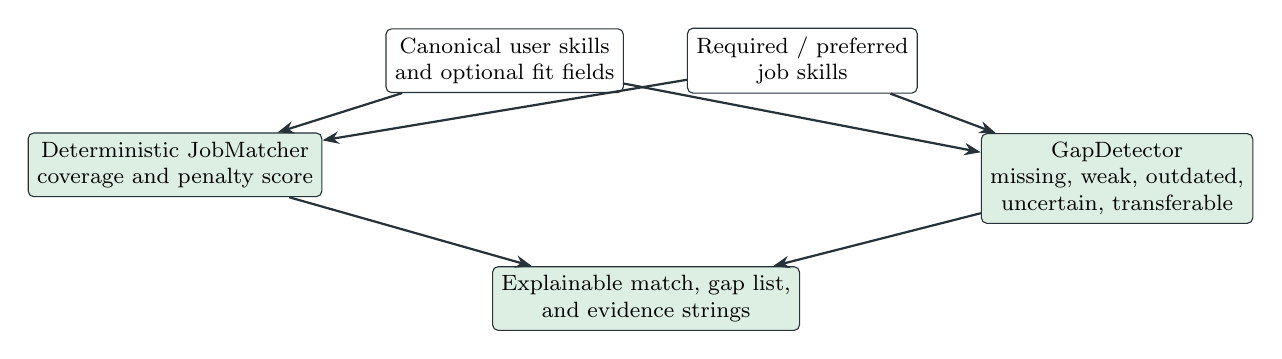
\begin{tikzpicture}[node distance=5mm and 8mm]
\node[data] (profile) {Canonical user skills\\and optional fit fields};
\node[data,right=of profile] (job) {Required / preferred\\job skills};
\node[impl,below left=of profile] (match) {Deterministic JobMatcher\\coverage and penalty score};
\node[impl,below right=of job] (gap) {GapDetector\\missing, weak, outdated,\\uncertain, transferable};
\node[impl,below=12mm of $(match)!0.5!(gap)$] (out) {Explainable match, gap list,\\and evidence strings};
\draw[flow] (profile)--(match); \draw[flow] (job)--(match); \draw[flow] (profile)--(gap); \draw[flow] (job)--(gap); \draw[flow] (match)--(out); \draw[flow] (gap)--(out);
\end{tikzpicture}

\caption{Implemented deterministic matching and gap-detection flow. Optional semantic, experience, and preference fit fields are caller-supplied rather than learned by the repository.}
\label{fig:matching}
\end{figure}

The score must not be treated as a hiring prediction. Its weights are transparent implementation choices, not fitted parameters. The lack of labelled relevance data is especially important here: a high coverage score could still recommend a role that mismatches seniority, location, compensation, accessibility needs, or nuanced work experience. A responsible system would use this output as evidence-backed decision support and make the components visible, not as automatic eligibility screening.

\section{Course recommendation}

\inlinecode{CourseRecommender} accepts gap objects, a course catalogue, and an optional profile. It considers only courses that cover at least one gap. For each it calculates gap coverage, prerequisite fit, supplied level fit, supplied goal alignment, and workload penalty, then clips a weighted sum to $[0,1]$. The output includes course identifier/name, covered skills, gap-coverage fraction, a score, and a sentence explaining the covered gaps. This is a readable implementation of a rule-based baseline, and its unit test verifies a simple expected course.

\begin{figure}[H]
\centering
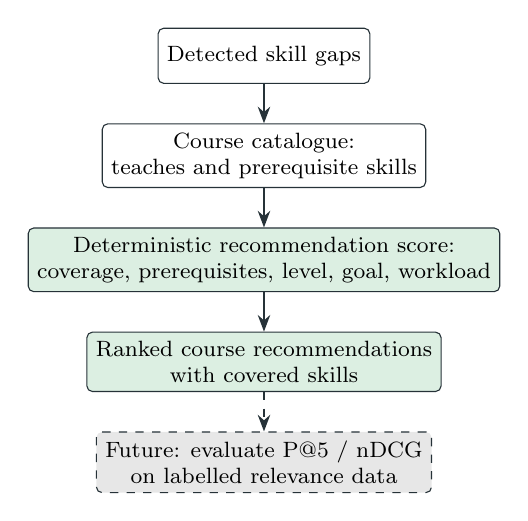
\begin{tikzpicture}[node distance=5mm]
\node[data] (gaps) {Detected skill gaps};
\node[data,below=of gaps] (catalog) {Course catalogue:\\teaches and prerequisite skills};
\node[impl,below=of catalog] (score) {Deterministic recommendation score:\\coverage, prerequisites, level, goal, workload};
\node[impl,below=of score] (rank) {Ranked course recommendations\\with covered skills};
\node[plan,below=of rank] (eval) {Future: evaluate P@5 / nDCG\\on labelled relevance data};
\draw[flow] (gaps)--(catalog); \draw[flow] (catalog)--(score); \draw[flow] (score)--(rank); \draw[dashedflow] (rank)--(eval);
\end{tikzpicture}

\caption{Implemented course-recommendation flow and its explicit evaluation boundary. P@5 is unavailable because no labelled course relevance data are persisted.}
\label{fig:course}
\end{figure}

The current catalogue inputs are demo data. No thesis claim is made about course quality, learner success, fairness, or P@5. A meaningful next evaluation would assemble user/job/course triples with independently judged relevant courses, ensure train/test separation where learned components are added, compare simple coverage ranking with stronger retrieval baselines, and analyse whether recommendations differ systematically across user groups. Until then, the recommender is an inspectable vertical-slice component rather than a validated intervention.

\section{A staged deployment interpretation}

The context and graph architecture suggests a safe future rollout. Stage one can expose extraction and canonicalization with evidence and correction affordances. Stage two can offer profile compaction, showing exactly what will be cached and allowing the user to add, remove, or dispute facts. Stage three can show deterministic gap and course suggestions as explanations, clearly labelled as unvalidated. Only after a labelled offline evaluation and a fairness/privacy review should the system use learned rankers or consequential matching decisions. This staged interpretation aligns the strength of a feature's claims with the strength of its evidence.

\chapter{Limitations, Threats to Validity, and Future Work}
\label{ch:limitations}

\section{Claim boundary}

This report is intentionally narrower than the codebase's conceptual scope. Its strongest quantitative evidence concerns span extraction and three wrapper variants. Its strongest engineering evidence concerns explicit schemas, source-preserving operations, unit tests, configuration, and persisted artifacts. The graph, profile, matching, and recommendation modules are implemented but do not have labelled effectiveness measures. \Cref{fig:status} summarises this boundary. A reader should treat it as part of the result, not as a caveat to skip.

\begin{figure}[H]
\centering
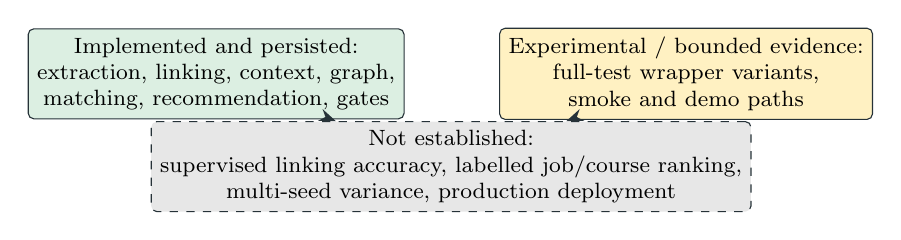
\begin{tikzpicture}[node distance=6mm and 12mm]
\node[impl] (implemented) {Implemented and persisted:\\extraction, linking, context, graph,\\matching, recommendation, gates};
\node[exp,right=of implemented] (experimental) {Experimental / bounded evidence:\\full-test wrapper variants,\\smoke and demo paths};
\node[plan,below=of $(implemented)!0.5!(experimental)$] (future) {Not established:\\supervised linking accuracy, labelled job/course ranking,\\multi-seed variance, production deployment};
\draw[dashedflow] (implemented)--(future); \draw[dashedflow] (experimental)--(future);
\end{tikzpicture}

\caption{Evidence status across SkillLLM\_v2. A complete vertical slice is not the same as a complete outcome evaluation.}
\label{fig:status}
\end{figure}

\section{Dataset and evaluation limitations}

SkillSpan is an English job-posting benchmark with expert hard/soft span annotation~\cite{zhang2022skillspan}. It is an appropriate starting point, but a strong score on this export does not establish transfer to resumes, course catalogues, conversational profile updates, or multilingual labour markets. The local data contain technical and house sources, and the selected training/evaluation transformation may differ from other published SkillSpan protocols. The full Mistral artifact reports a 974-document cached evaluation path although the local test JSON has 3,569 rows. The repository does not provide a sufficiently explicit manifest explaining that subset in this audit. That ambiguity is a reproducibility limitation and should be resolved before a final defence claim.

Exact span F1 is rigorous but incomplete. It penalises a boundary difference even when a human would consider the prediction useful, while partial and token metrics may make a boundary failure look less serious than it is for evidence display. No qualitative, blinded annotation study is stored to determine whether errors are concentrated in rare technologies, compositional skills, soft skills, source domains, or annotation ambiguities. The report also lacks confidence intervals and multi-seed runs. The observed 0.001-level wrapper differences could change under another seed or subset.

\section{Model and training limitations}

The persisted Mistral run is substantial: it uses an 80-epoch 4-bit LoRA configuration and two RTX 3090 GPUs. Nevertheless, it is a single run with stored losses and artifacts, not a hyperparameter or checkpoint-selection study. The reports do not establish a validation-selected epoch, compare LoRA ranks, test prompt variants, or provide a full ablation of quantization and distributed settings. The extractor has a deterministic smoke fallback; although the primary metric says fallback was false, every future run must preserve that check. A model-loading issue could otherwise turn a seemingly valid model result into a keyword baseline.

The Mistral adapter assigns a fixed candidate confidence in its extraction adapter. The confidence calibrator uses rules and thresholds, but no calibration curve, expected calibration error, or probability-quality assessment is persisted. Confidence should therefore be read as a gating/control signal, not as a statistically calibrated belief. The same caveat applies to verifier outputs and matcher scores.

\section{Normalization and ontology limitations}

The local alias table has 696 canonical entries and produces high attachment coverage in the stored wrapper reports. Coverage is not correctness. Gold canonical labels, a validated taxonomy version, hierarchy-aware scoring, and error analysis by taxonomy source are required before making a canonical-link accuracy claim. The code has loaders for ESCO, O*NET, Lightcast, and custom data, but the reported setup uses custom aliases. External taxonomy licenses, versions, semantic drift, and alias collisions would need governance in a production setting.

Attach-only normalization is deliberately conservative, but it creates a trade-off. It protects extraction metrics from a bad link, while an incorrect canonical field can still mislead matching, aggregation, or graph paths. A future linker should keep candidate alternatives, calibration/evidence scores, taxonomy provenance, and user correction history rather than pretending that one alias match is definitive.

\section{Context, graph, and recommendation limitations}

The profile summary preserves supplied evidence but does not model recency, proficiency, evidence reliability, temporal contradiction, or user consent beyond the input interface. It must not be populated from sensitive personal attributes or used to infer protected characteristics. The cache hash detects a payload change but does not solve cache invalidation, retention policy, access control, encryption, deletion requests, or cross-device synchronisation. The current CAG/RAG separation is a software policy rather than a measured reduction in token use, latency, hallucination, or retrieval error.

The graph is in memory and its relation vocabulary is manually constructed. It does not provide transactional updates, scalable storage, graph embeddings, learned edge confidence, or a formal provenance model for derived edges. The matcher and course recommender use hand-specified weights. They have no nDCG, P@5, calibration, fairness, or user-satisfaction result. A job match score must never be used as an automated hiring, admission, or eligibility decision. Any serious deployment would require human oversight, an appeal/correction route, data minimisation, and a fairness evaluation that is appropriate to the intended population.

\section{Reproducibility and report-format limitations}

The Stage-2 branch has no commits. The artifact directory preserves useful evidence but cannot by itself establish exactly which source revision created every output. Timestamp-based provenance checking is helpful but vulnerable to copied files and does not hash all dependencies. The environment description is partial: Python, PyTorch/CUDA, hardware, and YAML values are available, while a complete lock file, container, dataset fingerprint, and immutable experiment registry are not. The report's new figures are reproducible TikZ source, but the final institutional format still needs the author, official course designation, committee, and template confirmation. It is not a substitute for SFSU Graduate Studies approval.

\section{Future work}

The most valuable next step is a versioned, labelled evaluation program rather than another unmeasured architectural module. First, commit the Stage-2 source, record dataset hashes and the exact 974-document evaluation manifest, and rerun the primary experiment across multiple seeds. Report mean, dispersion, and paired wrapper tests. Second, create a canonical-link dataset with gold IDs and evaluate both coverage and accuracy; preserve alternate candidates and test long-tail aliases. Third, collect job/profile and course/gap relevance labels, define privacy and consent rules, and evaluate matching and recommendation with nDCG, P@5, coverage, calibration, and subgroup error analysis.

On the modelling side, investigate soft-skill errors by span length, annotation source, and semantic category. Compare the fixed prompt with controlled variants, examine calibration, and conduct a proper boundary-refiner ablation that logs every edit. On the systems side, extend profile facts with temporal evidence and user-confirmed proficiency while preserving the original sources; introduce a versioned graph store and explicit derived-edge provenance; and replace the lexical retrieval demo with evaluated sparse, dense, and hybrid baselines. Each addition should remain behind the same anchor-preserving and artifact-provenance controls that produced the central finding of this report.

\chapter{Conclusion}
\label{ch:conclusion}

SkillLLM\_v2 demonstrates a complete, evidence-aware path from span-level skill extraction to canonicalized profile, contextual packet, graph, gap, and course-recommendation records. Its principal measured result is the persisted 80-epoch Mistral LoRA extractor: exact-span F1 0.670069, token F1 0.787886, hard-skill F1 0.726450, and soft-skill F1 0.604046 in the audited Stage-2 artifact. The included BERT and zero-shot GLiNER artifacts are far lower under the same local reporting path. Within this repository, the adapted Mistral model is consequently the correct extraction anchor.

The system's more important design result is negative and constructive at once. Historical wrapper analysis showed that boundary edits and verifier rejection could substantially damage correct anchor spans. The current architecture responds with Mistral-source protection, add-only auxiliary candidates, attach-only linking, and a non-regression gate with explicit fallback. The later safe-wrapper artifacts remain close to the anchor and are accepted under their configured floors, but their thousandth-scale metric differences do not establish a general accuracy gain. The report therefore rejects the premise that more downstream components automatically make extraction better.

The remaining modules are useful because they enrich rather than replace evidence. A canonical identifier can be attached without changing the original span. A profile fact can retain its source, offset, confidence, and conflict note. A cached packet can separate stable information from dynamic job text. A graph and deterministic score can make a gap or course recommendation inspectable. These features are implemented and tested as a vertical slice. They are not yet evidence that the system matches jobs or recommends courses effectively, fairly, or safely.

Next work should version inputs, repeat extraction across seeds, and add gold labels. Until then, extraction provenance remains the central invariant.

\appendix
\chapter{Reproducibility Record}
\label{app:reproducibility}

This appendix records the local paths and conditions needed to inspect or reproduce the claims in this report. It is intentionally not a promise that every command will run unchanged on another machine. The source tree has no commit at the audited branch, large model files are local, and the report has no container or lock-file artifact. A future reproducibility release should address those gaps.

\section{Environment evidence}

The run manifest at \codepath{SkillLLM\_v2\_stage2/reports/skillllm\_v2/research\_refresh/run\_manifest.json} records Linux, Python 3.12.3, PyTorch 2.6.0+cu124, CUDA availability, and two NVIDIA GeForce RTX 3090 devices with 24 GiB memory each. The training summary at \codepath{artifacts/skillllm\_v2/mistral\_lora/model/training\_summary.json} records world size 2 and epoch 80. The active full-run YAML is \codepath{configs/skillllm\_v2\_training\_80ep\_2gpu.yaml}. These artifacts describe the recorded run; any new run should write a fresh manifest rather than inheriting this metadata.

The package list in \codepath{requirements.txt} names PyTorch, LLaMA-Factory, GLiNER, NetworkX, scikit-learn, YAML, and related libraries. It is not a complete platform lock. In particular, the exact CUDA driver, compiler, PyPI resolution, installed Git dependency commits, tokenizer assets, and model download state should be captured in a future environment manifest.

\section{Data and source checkpoints}

The dataset root is \codepath{data/source/skillspan\_hf/}. Its three JSON files have 4,800, 3,174, and 3,569 lines for train, development, and test. The dataset README contains its attribution and licence. Before a rerun, record a SHA-256 fingerprint of each JSON file and a manifest identifying the 974-document evaluation path used by the cached Mistral artifacts. This report does not reconstruct that subset because the current artifacts do not explain it sufficiently.

The Mistral training code is \codepath{src/skillllm\_v2/train/mistral\_lora\_trainer.py}; SFT data construction is \codepath{src/skillllm\_v2/train/build\_mistral\_sft\_data.py}. The primary adapter/checkpoint assets are stored under \codepath{artifacts/skillllm\_v2/mistral\_lora/model/}. \inlinecode{training_summary.json} identifies the model path as \codepath{models/mistral-small-3.1-24b-instruct-2503}. This report never modifies any of those model or experiment artifacts.

\section{Representative commands}

The repository's shell scripts provide the authoritative launch interfaces. The following commands are representative inspection and validation commands; they should be run from the Stage-2 root after activating a compatible project environment and setting `PYTHONPATH=src`.

\begin{verbatim}
cd "/home/923873155/Sem 4 Research/SkillLLM_v2_stage2"
export PYTHONPATH=src
export CUDA_VISIBLE_DEVICES=0,1
export TOKENIZERS_PARALLELISM=false
export WANDB_DISABLED=true

pytest -q tests/skillllm_v2 tests/test_skillllm_v2_stage2.py
python -m skillllm_v2.eval.prediction_provenance_check
python -m skillllm_v2.eval.run_safe_wrapper \
  --config configs/skillllm_v2_training_80ep_2gpu.yaml
\end{verbatim}

The final command re-evaluates wrapper components against cached anchor predictions; it does not retrain Mistral. Training is consequential GPU work and should be launched only through the project scripts/configuration after confirming model paths, storage, and a fresh experiment ID. The report's metrics are the persisted historical artifacts, not outputs generated while typesetting this document.

\section{Artifact verification sequence}

The following sequence maintains the report's claim boundary:

\begin{enumerate}
  \item Inspect the configuration, data paths, and model/training summary.
  \item Confirm that primary Mistral `metrics.json` says fallback was false.
  \item Read the primary prediction and metric artifacts before generating tables.
  \item Run the provenance check and preserve its output with the report revision.
  \item Treat any status file ending in or describing a smoke operation as smoke evidence only.
  \item Regenerate wrapper metrics on the same manifest before comparing a code change with the anchor.
  \item Version source, configuration, dataset fingerprints, and generated tables together before external release.
\end{enumerate}

\section{Tests and their interpretation}

The focused test suite covers schemas, Mistral SFT-data construction, BERT/GLiNER smoke paths, candidate merging, boundary refinement, calibration, taxonomy linking, profile summarisation, cached context, graph construction, job matching, course recommendation, pipeline gates, and non-regression selection. A current report-verification run passed 50 tests in 1.34 seconds under Python 3.13.12. That runtime is separate from the recorded training environment. A passing unit test demonstrates an invariant or small example; it does not replace the full-test extraction metrics, linking labels, ranking labels, or a deployment evaluation. The distinction should remain visible in automated continuous integration as well as in the thesis.

\chapter{Prompt and Data-Contract Details}
\label{app:prompt-schema}

\section{Extraction prompt design}

The Mistral extractor uses a system message stating that it identifies explicit skill spans from resumes, job postings, and professional text and must return valid JSON only. The user prompt then directs the model to extract exact surface spans, forbid paraphrase and unstated inference, include technical and soft skills only when explicitly mentioned, ignore titles and generic responsibilities unless explicitly skills, and use an empty list when no skills occur. It asks for objects with `text` and `label` fields.

The training renderer constructs the assistant target from the local gold spans as compact JSON. It uses the text and label but not the offset in the target. This means that source alignment is not delegated to the model output schema: after generation, \inlinecode{find_offsets} locates the predicted text in the input and the validator confirms a coherent candidate. The design is conservative. A model output that paraphrases a true skill is not silently credited as an exact span.

\section{Skill candidate contract}

The following abstract JSON record mirrors \inlinecode{SkillCandidate.to_dict()} and its validator. It is a representation schema, not a record copied from a user.

\begin{verbatim}
{
  "surface_form": "Python",
  "label": "HARD_SKILL",
  "start": 18,
  "end": 24,
  "source": "mistral",
  "confidence": 0.86,
  "evidence": "experience with Python and SQL",
  "canonical_skill_id": "optional-id-or-null",
  "canonical_skill_name": "optional-name-or-null",
  "metadata": {
    "raw_label": "HARD_SKILL"
  }
}
\end{verbatim}

The validator restricts labels to \inlinecode{HARD_SKILL} and \inlinecode{SOFT_SKILL}, source to \inlinecode{bert}, \inlinecode{mistral}, \inlinecode{gliner}, or \inlinecode{dictionary}, confidence to the inclusive interval $[0,1]$, and offsets to a valid pair. A merger can add \inlinecode{metadata.sources} to show that several candidates support the same retained record. A linker can fill canonical fields. Neither operation should erase the original source information.

\section{Profile and context contract}

\inlinecode{ProfileSummary} stores a user identifier, generation time, an ordered list of skill facts, target roles, missing skills, course history, preferences, and conflict notes. A fact stores a confidence and one or more \inlinecode{Evidence} items. The cached context packet supplies packet type, cache policy, payload, and content-hash fields. Its policy contains three lists:

\begin{verbatim}
cag:   profile_summary, skill_memory, taxonomy_aliases, course_catalog_summary
rag:   job_postings, scraped_descriptions
graph: user_skill_job_course_paths
\end{verbatim}

This schema states which category an item belongs to; it does not by itself implement database persistence, authorization, or automatic invalidation. Applications consuming it should surface user controls and treat the hash as an integrity/debugging aid rather than a security boundary.

\section{Matching and recommendation output contract}

The job matcher returns a job identifier, a score in $[0,1]$, matched skills, missing skills, critical missing skills, evidence strings, and a short explanation label. The gap detector emits a list of skill/gap-type pairs. The course recommender returns a course identifier/name, skills it covers, a gap-coverage ratio, a score, and a reason. These outputs contain transparent intermediate values, which is preferable to a bare score in a research prototype. They should not be interpreted as a decision on employment eligibility or a statement of a user's competence.

\chapter{Audit Trail and Artifact Index}
\label{app:audit}

\section{Primary source of truth}

The detailed audit is maintained outside the PDF at \codepath{docs/thesis/codebase\_audit.md}. It describes the branch state, source modules, configurations, data counts, persisted metrics, historical conflict, test coverage, and claim boundary. This appendix provides a compact index so that a committee member can locate the evidence behind each main result without relying on an informal narrative.

\begin{longtable}{p{0.27\textwidth}p{0.31\textwidth}p{0.31\textwidth}}
\caption{Claim-to-artifact index.}\label{tab:artifact-index}\\
\toprule
Claim & Primary local evidence & Interpretation limit \\
\midrule
\endfirsthead
\toprule
Claim & Primary local evidence & Interpretation limit \\
\midrule
\endhead
Mistral extraction F1 & \codepath{artifacts/skillllm\_v2/mistral\_lora/metrics.json} & One persisted evaluation snapshot; no multi-seed estimate \\
Mistral training & \codepath{mistral\_lora/model/training\_summary.json} & Records runtime/loss/world size, not global optimality \\
BERT and GLiNER baselines & Their respective \codepath{metrics.json} files & CPU-fast and zero-shot qualifications apply \\
Safe-wrapper decision & \codepath{safe\_wrapper/metrics.json} and \codepath{safe\_wrapper\_gate.md} & Tolerance-based compatibility, not statistical superiority \\
Historical regression & \codepath{wrapper\_error\_analysis.md} & Older diagnostic; not pooled with later table \\
Linking coverage & \codepath{mistral\_gliner\_taxonomy/metrics.json}; \codepath{full\_cag\_graph/metrics.json} & Coverage is not supervised linking accuracy \\
Profile/context path & \codepath{context/*.json}; context source/tests & Smoke-tested structured data flow \\
Graph/matching/course path & \codepath{demo/*.json}; source/tests & nDCG@10 and P@5 unavailable \\
Artifact ordering & \codepath{prediction\_provenance\_check.md} & Timestamp check, not immutable lineage \\
Hardware/runtime & \codepath{research\_refresh/run\_manifest.json} & Describes recorded environment only \\
\bottomrule
\end{longtable}

\section{Known metric conflict}

Two source families contain different anchor values. The historical error report uses 0.675034 exact F1 and 0.609792 soft F1 for an earlier anchor. The later primary Mistral `metrics.json` uses 0.670069 and 0.604046. This report uses the later persisted metrics for the main table because they are the artifacts selected by the current money table, sanity report, safe-wrapper metrics, and provenance check. It retains the earlier report only to explain the failure mode that motivated source-aware policy and gate design. No average, difference, or ranking in this thesis mixes the two source families.

\section{Report maintenance checklist}

Before submitting a revision, regenerate tables from the current metric artifacts; rebuild the PDF; update the audit with any changed path or metric; rerun the garbage-text scan; verify every figure/table reference; and update the administrative cover-page details only after the department confirms the final route and template. If a new model run changes the anchor, regenerate every wrapper comparison rather than copying the previous threshold. If labelled downstream data become available, add a separate evaluation chapter/table rather than rewriting the current smoke/demo claims.


\bibliographystyle{plain}
\bibliography{references}
\end{document}
